\documentclass{article}
\usepackage[utf8]{inputenc}
\usepackage{hyperref}
\usepackage[superscript]{cite}
\usepackage{amsmath}
\usepackage{graphicx}
\graphicspath{ {./images/} }
\usepackage[export]{adjustbox}
\usepackage{blindtext}
\usepackage{geometry}
\usepackage{tabularx}
% \usepackage[table]{xcolor}
\usepackage{caption}
\usepackage{subcaption}
 \geometry{
 a4paper,
 total={170mm,257mm},
 left=20mm,
 top=20mm,
 }
 \usepackage{parskip}
 \usepackage{color, colortbl}

\title{ISYE 6748 Applied Analytics Practicum \\
Fortiphyd Logic: Anomaly Detection in Industrial Control Systems}
\author{Krishna Kumar and Sumit Machwe}
\date{Fall 2022}

\begin{document}
\maketitle

\tableofcontents
\definecolor{x11gray}{rgb}{0.75, 0.75, 0.75}
\definecolor{applegreen}{rgb}{0.55, 0.71, 0.0}

\section{Introduction}
\setlength{\parskip}{5pt}
\leftskip 10pt
Goal of this project is to devise generalizable anomaly detection in industrial control system sensor data. Fortiphyd Logic is a cybersecurity startup firm that specializes in fortifying industrial networks from malicious cyber attacks. \par
According to the paper\cite{one} written by the firm's founder, David Fromby, most of the industrial IoT device infrastructure (programmable control logic devices) is vulnerable to cyber-attacks and may result in massive economic losses. \par
Early detection of such attacks can not only save critical time to recovery but also encourage the PLC manufacturing companies to implement better security controls around the devices and prevent value loss. \par
For this project, we analyze the sensor data from a scaled-down version of an industrial water treatment plant. The plant consists of six stage filtration process. Water was continuously run for 11 days through the system. Network and physical attacks were launched during this period. The data consists of physical properties related to the plant and treatment process as well as network traffic data. Data files consist of non-anomalous and anomalous data. Please refer to this paper for further details\cite{two}.\par

\section{Approach}

Developing a generic anomaly detection process is hard. Unfortunately, one model fits all does not apply, especially when we do not want to incorporate domain knowledge about the dataset. We can however develop a framework that can be applied to other use cases with reasonably minimal changes. The approach we took required not to delve into the physics (or chemistry) of the dataset, but rather identify dependent variables that can be used to describe normal state behavior over time and which can be used in building unsupervised learning model.\par

In pursuit of such an approach, we discovered `pycaret' library which organizes various Anomaly Detection algorithms. Under the hood, it uses `PyOD' open-source library. \par

\subsection{Solution outline}
\begin{enumerate}
    \item Prepare data for analysis and feature selection. Please refer to section \ref{EDA} and \ref{featureSelection}
    \item Partition training data vertically across 6 sub-systems.
        \begin{equation}
            \begin{aligned}
                S &= \{P_1, P_2, P_3, P_4, P_5, P_6\} \\
                M &= \{\text{OCSVM, iforest, Histogram, KNN, LOF, MCD}\} \\
                \text{Number of Models} &= S \times M = 6 \times 6 = 36 \\
                \text{Models not Built}^{\ref{infraLimit}} &= 8 \\
                \text{Total Models Built} &= 36 - 8 = 28
            \end{aligned}
        \end{equation} 
    \item Performance Metrics 
    %TODO: KK to provide def for "Identified Attack %" and "Propensity of attack"
    %TODO: Make sure to list sigma 1.0 and 0.5 measures 
    \item \textit{Why not produce confusion matrix?} \par
    Because we have used an expansionary definition of actual attacks. Please refer to assumption section \ref{Assumptions}

    \item Analyze and conclude the findings. The objective is to find the best-performing model and model group based on performance matrices. Please refer to section \ref{analysisConclusion}.
    
    \item key design decisions:
    \begin{enumerate}
        \item \textbf{Unsupervised} algorithm is preferred even though we have labeled data. In order to develop a generalizable anomaly detection approach, we do not emphasize on number or attributes of parameters.
        \item We have also used one of the \textbf{supervised} learning approaches `KNN' in order to seek better performance with labeled data. 
    \end{enumerate}
    % TODO: KK has to add description why 2 alogs did not work
    % TODO: Provide hardware profile (Google Collab's CPU and Memory. Local machine  etc.)
    
\end{enumerate}

\subsection{Assumptions} \label{Assumptions}
Following assumptions apply to our implementation of Anomaly Detection:
\begin{enumerate}
    \item \textbf{Actual attack data identifier}: It is difficult to isolate sensor malfunction from a malicious attack. Without sufficient data knowledge, it is difficult to identify actual attacks in the given attack period. Hence we decided that every record in a given attack window is an actual attack.

    \item \textbf{Data Partitioning}: The given SWaT training dataset is relatively large (495000 records, 53 features). Subjecting this data to train underlying models could not succeed due to memory constraints. 
    In order to overcome memory issues, and in discussion with project sponsors: 
    \begin{enumerate}
        \item \textbf{Partition training data by days [22-Dec-2015 to 28-Dec-2015]}. However, due to reduced training data the models could not provide acceptable performance. The percentage of identified attacks for OCSVM model was around \textit{19\%}.
        %TODO: Add evidence
        \item \textbf{PCA and Multicollinearity}: To reduce feature space, we applied principal component analysis upto 10 dimensions. However, training could not succeed since PCA is a highly memory-intensive process. \textit{However, given better infrastructure, we recommend applying PCA.} \\
        Our EDA highlighted the correlation between sensors and actuators. We tried removing multicollinearity to retain statistical significance. However, we faced memory constraints while removing multicollinearity during training. \textit{However, given better infrastructure, we recommend removing multicollinearity.}
        
        \item \textbf{Partition training data by sub-systems}. Our assumption for this approach is that each sub-system can be analyzed independently and there are negligible interactions across sub-systems. We chose this approach as we could get significantly better results. The percentage of identified attacks for OCSVM model was around \textbf{91\%}.          
    \end{enumerate} 
    
    \item \label{infraLimit} \textbf{Infrastructure Limitations}: Our conclusions and results are based on analyzing all sub-systems except:
    %TODO Sumit REFORMAT - Done
    $$
    \begin{aligned}
        \textbf{OCSVM} &: \{ \text{$P_3$, $P_4$, $P_5$, $P_6$}  \} \\
        \textbf{$P_4$} &: \{ \text{MCD, Histogram, KNN, LOF} \}   \\     
    \end{aligned}    
    $$
    \begin{itemize}
        \item One class SVM model takes a long time to build on `Google Colab Pro'. We were able to build the OCSVM models for $P_1$ and $P_2$ sub-systems. However, models for other sub-systems failed due to memory constraints.
        \item For some reasons still unknown to us, 4 models for $P_4$ sub-systems could not be built due to memory constraints.
        \item Due to memory constraints, we could not perform PCA or remove multicollinearity. However, based on our EDA analysis, we recommend doing both. 
    \end{itemize}
    
    This may cause bias in our analysis and conclusions.    

\end{enumerate}

\subsection{Exploratory Time series Data Analysis} \label{EDA}
\subsubsection{Data Distribution}
    We reviewed the sensor and actuator data from various stages of the water treatment plant. The below plot (Figure \ref{fig:histogram}) shows data distribution of numeric features for all subsystems.
    \begin{figure}[!ht]
            \caption{Subsystem Sensors ${P_1, P_2, P_3, P_4, P_5, P_6}$ - Data Distribution Histogram}
            \label{fig:histogram}
                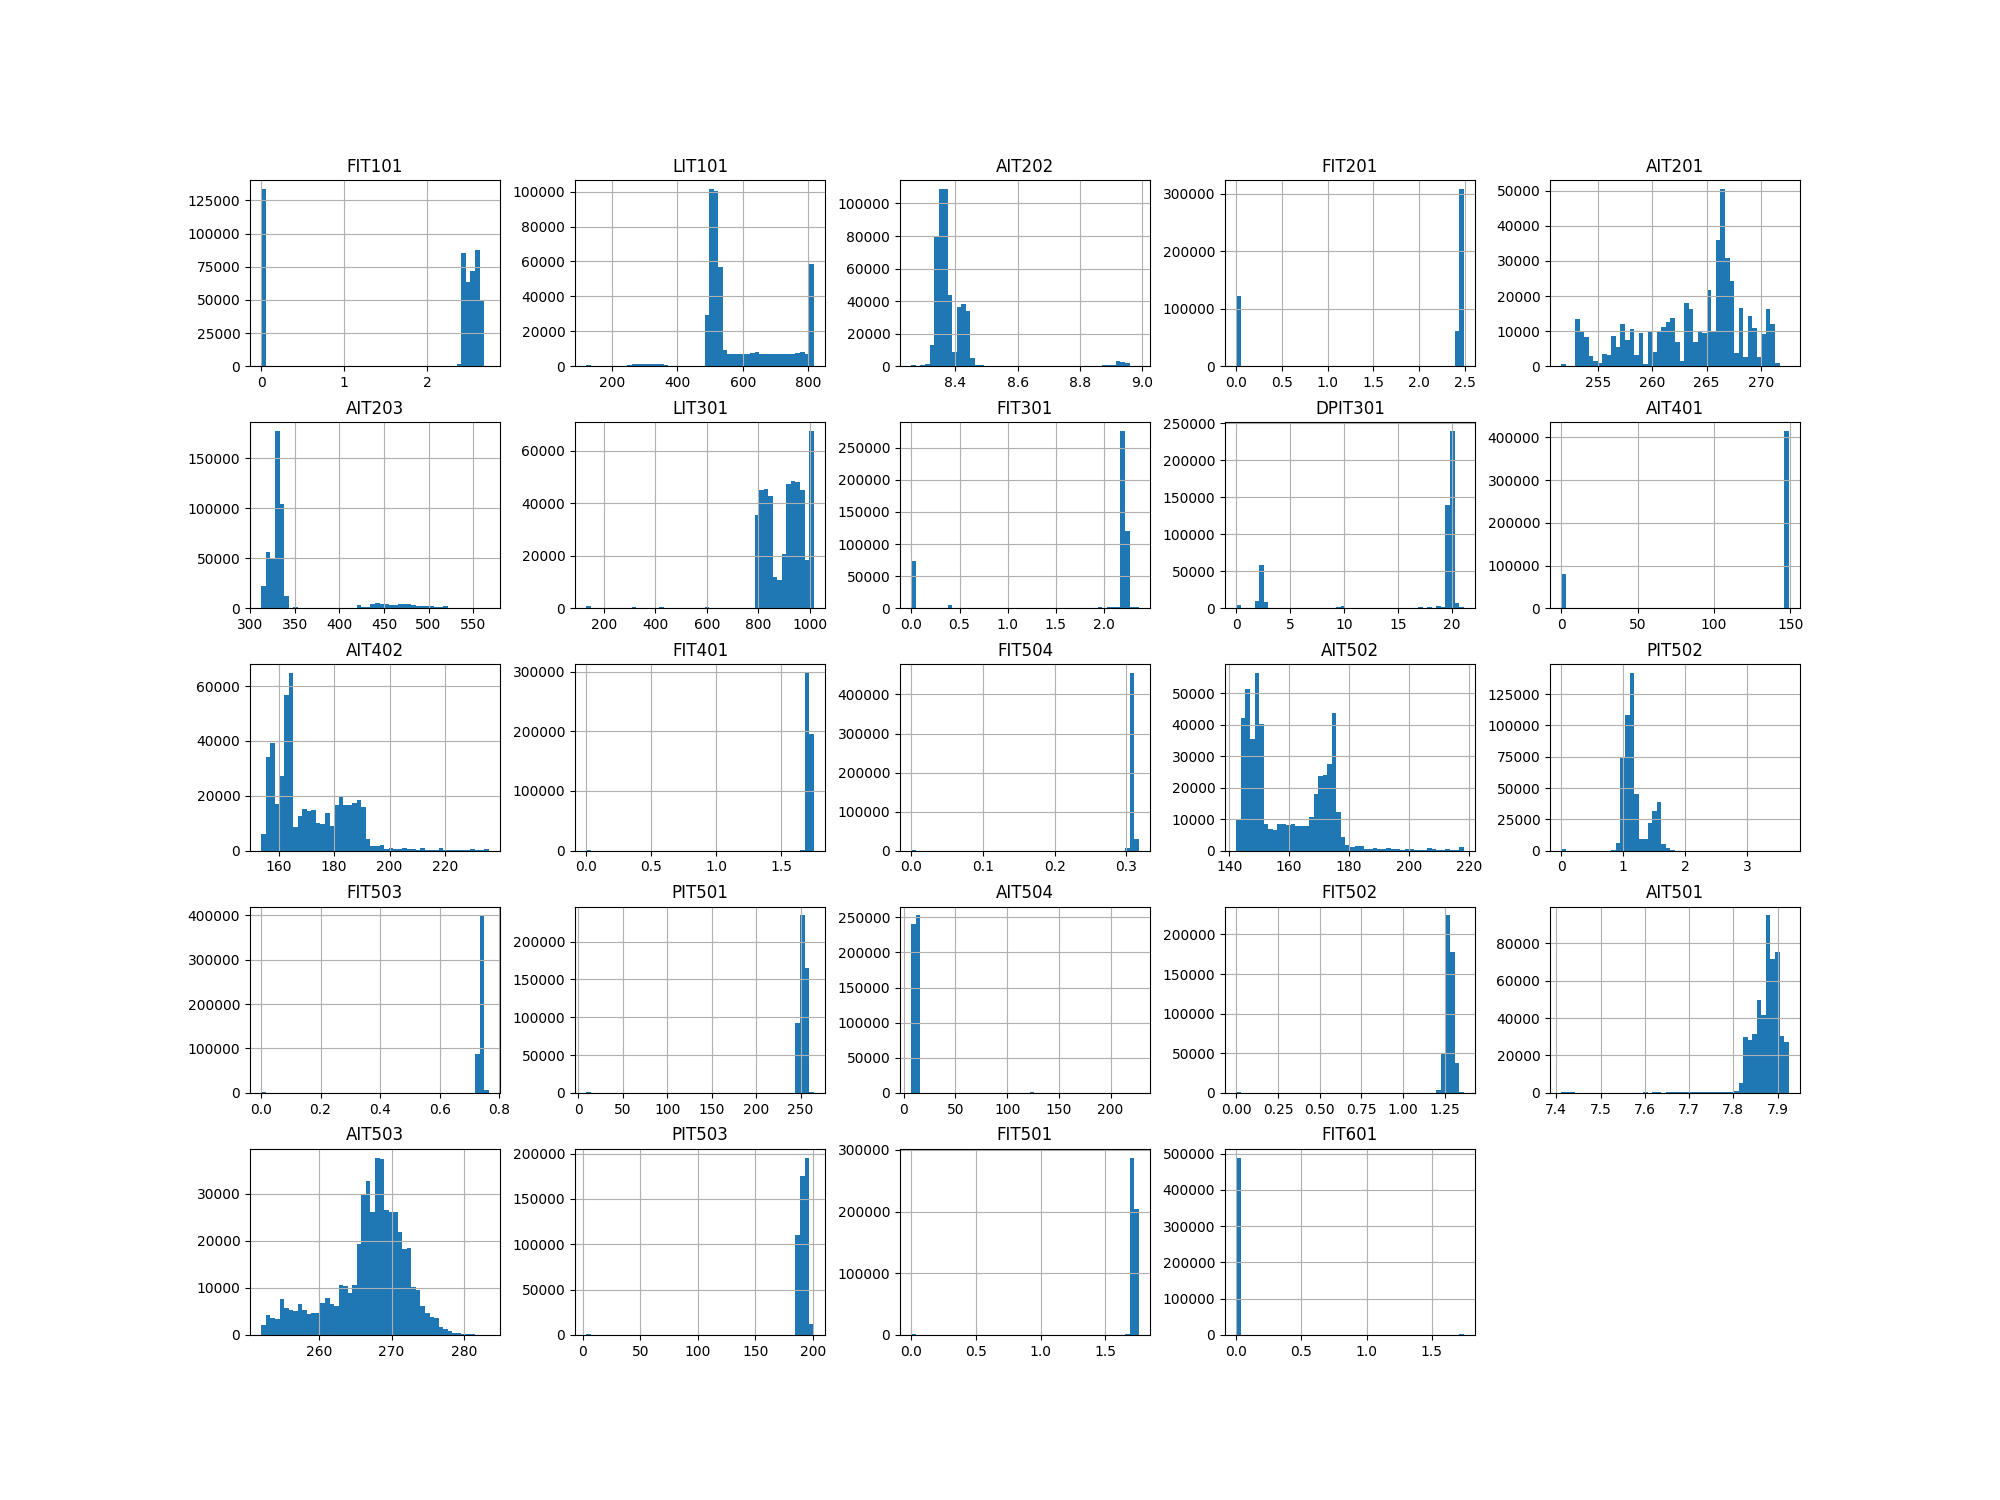
\includegraphics[width=0.9\textwidth]{images/EDA/NormalDataAllNumCols.png}
    \end{figure}

    The data distribution shows the multi-modal normal distribution with long tails for $FIT101$, $UT101$, $AIT202$, $AIT201$, $AIT203$, $LIT301$, $AIT402$, $AIT502$, $PIT502$, $AIT501$, and $AIT503$. Specific sub-systems such as $FIT501$, $FIT601$, $FIT401$, $FIT504$, and $AIT504$ do not seem to have Gaussian distribution as data distribution is concentrated to specific ranges. Based on the large data size, we can reasonably assume a normal distribution (Based on Central Limit Theorem - Gaussian Mixture model - Maximum Likelihood Probability). It is possible to transform the data to see if it has an unbiased normal distribution - but we decided not to do it and proceed with modeling.

\subsubsection{Heatmap}
    For each sub-system, we  created a correlation heatmap to determine if the sensor/actuator data are correlated. If they are highly correlated, we may decide to do dimensionality reduction using PCA (Principal Component Analysis). Please refer to the below plot (Figure \ref{fig:heatmap}) for the correlation Heatmap across subsystems 
    \begin{figure}[!ht]
        \caption{Subsystem Sensors ${P_1, P_2, P_3, P_4, P_5, P_6}$ - Correlation Heatmap}
        \label{fig:heatmap}
            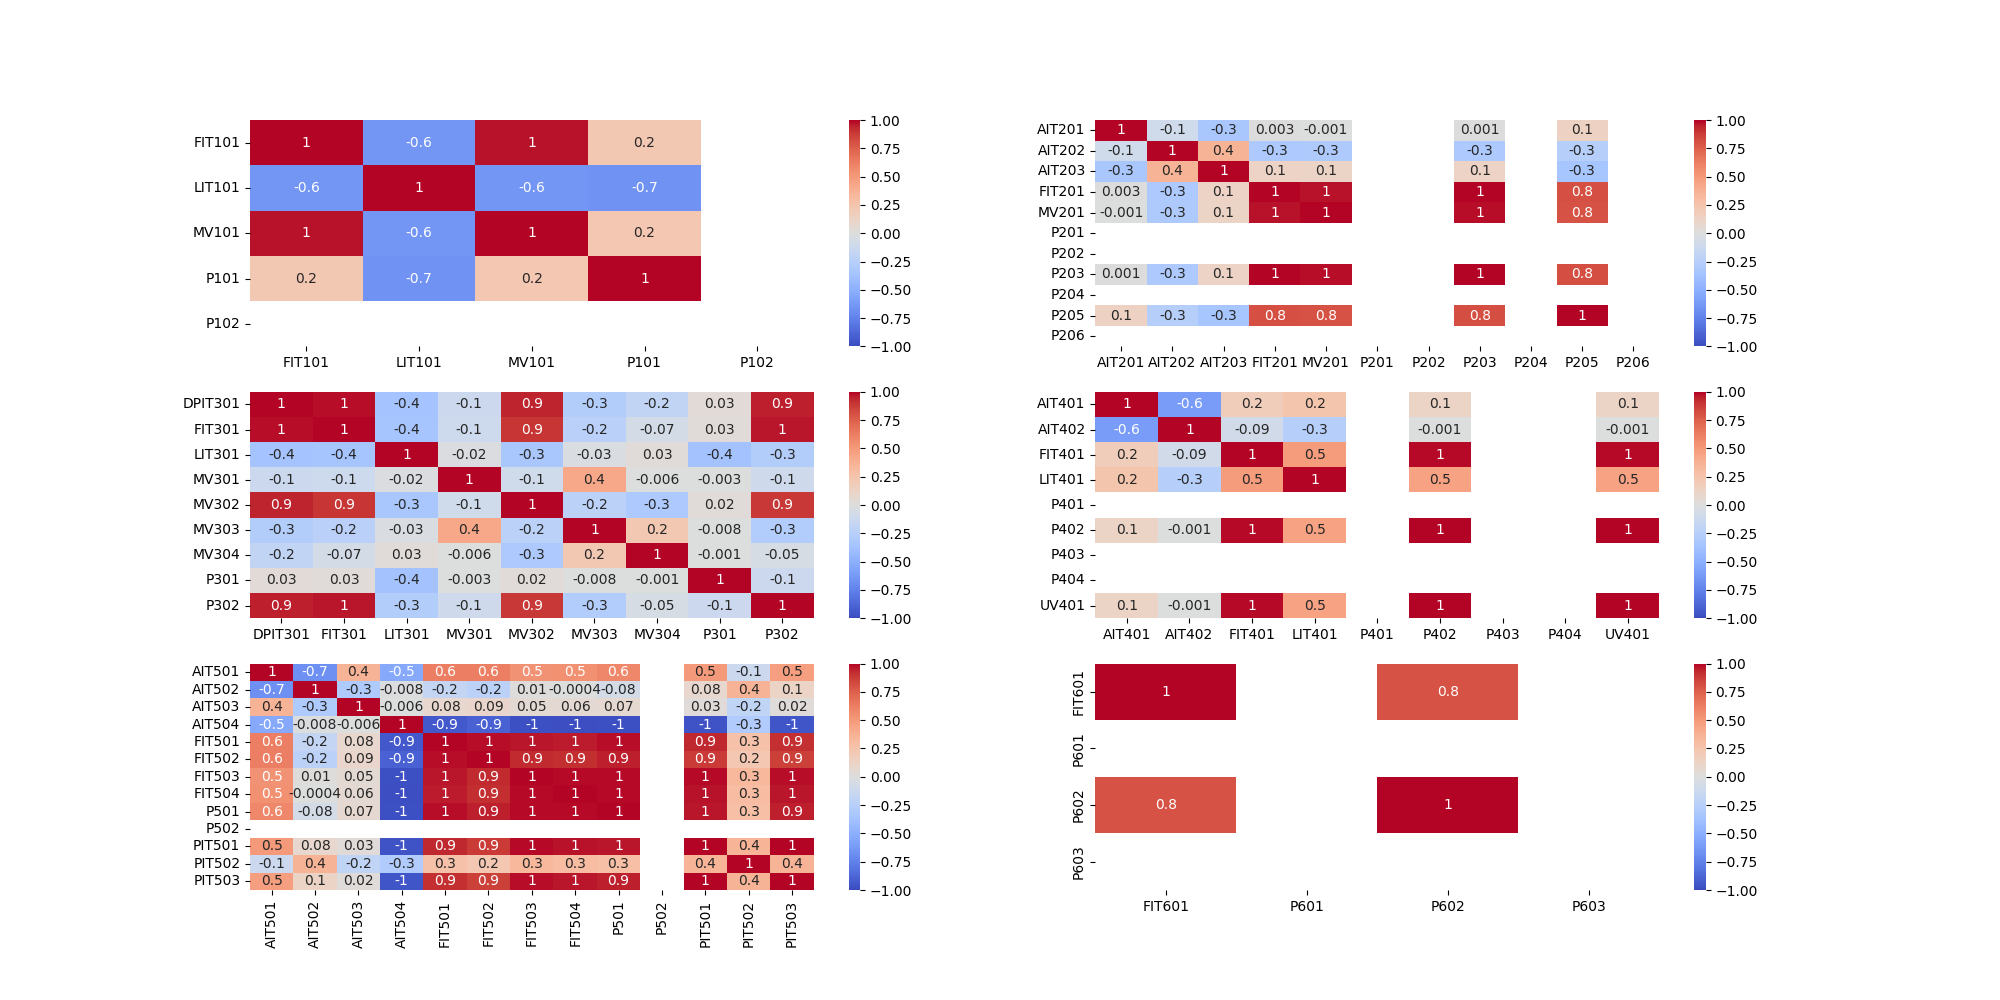
\includegraphics[width=1.0\textwidth]{images/EDA/AllSubSystemHeatMap.png}
    \end{figure}
    Based on the correlation Heatmap, we can conclude  that specific features within subsystems (for example $FIT101$ \& $LIT401$, $FIT201$ \& $P203$, $FIT301$ \& $P302$, $FIT401$ \& $P206$, $FIT501$ \& $FIT502$, $FIT601$ \& $P602$) are highly correlated. We should use PCA and remove multicollinearity while modeling. \cite{infraLimit}   
\clearpage
\subsubsection{Sub System Breakup}
    \begin{table}[!ht]  
            \begin{tabular}{|c|p{4cm}|p{4cm}|p{4cm}|}\hline
            \rowcolor{x11gray}
            \textsf{sub system} & \textsf{continuous variables} &  \textsf{categorical variables (actuators)} & \textsf{Ignore (constants)} \\ \hline            
            $P_1$ &{\small $FIT101$, $LIT101$, $MV101$, $P101$, $P102$} &{\small$MV101$, $P101$, $P102$} & {\small $P102$} \\ \hline
            $P_2$ &{\small $AIT201$, $AIT202$, $AIT203$, $FIT201$, $MV201$, $P201$, $P202$, $P203$, $P204$, $P205$, $P206$} &{\small$MV201$, $P201$, $P202$, $P203$, $P204$, $P205$, $P206$} &{\small$P201$, $P202$, $P204$, $P206$} \\ \hline
            $P_3$ &{\small $DPIT301$, $FIT301$, $LIT301$, $MV301$,$MV302$, $MV303$, $MV304$, $P301$, $P302$} &{\small$MV301$, $MV302$, $MV303$, $MV304$, $P301$, $P302$} & \\ \hline
            $P_4$ &{\small $AIT401$, $AIT402$, $FIT401$, $LIT401$, $P401$, $P402$, $P403$, $P404$, $UV401$} &{\small $LIT401$, $P401$, $P402$, $P403$, $P404$, $UV401$} &{\small$P401$, $P403$, $P404$} \\ \hline
            $P_5$ &{\small$AIT501$, $AIT502$, $AIT503$, $AIT504$, $FIT501$, $FIT502$, $FIT503$, $FIT504$, $P501$, $P502$, $PIT501$, $PIT502$, $PIT503$} &{\small$P501$, $P502$} &{\small $P502$}  \\ \hline
            $P_6$ &{\small $FIT601$,$P601$, $P602$, $P603$} &{\small $P601$, $P602$} &{\small $P601$, $P603$} \\ \hline
            \end{tabular}
        \caption{\textsf{Partition SWaT Dec 2015 spreadsheet into 6 sub systems} \\
            {\small \textsf{Ignore (Constants): Based on data analysis, these variables were found to have constant values and would not contribute to describing the variance in the model. They can be removed from the model-building exercise.}}}   
    \end{table}


\clearpage 

\subsubsection{Visualize Normal Data by sub-systems}
Visualizing training and test data is essential for analysis. Below graphs plot the continuous (Sensor data) and categorical (actuator data) variables on a log scale. Data being plotted is the mean value over 1 minute interval. Original data is provided at per second granularity.
    \begin{figure}[!ht]
        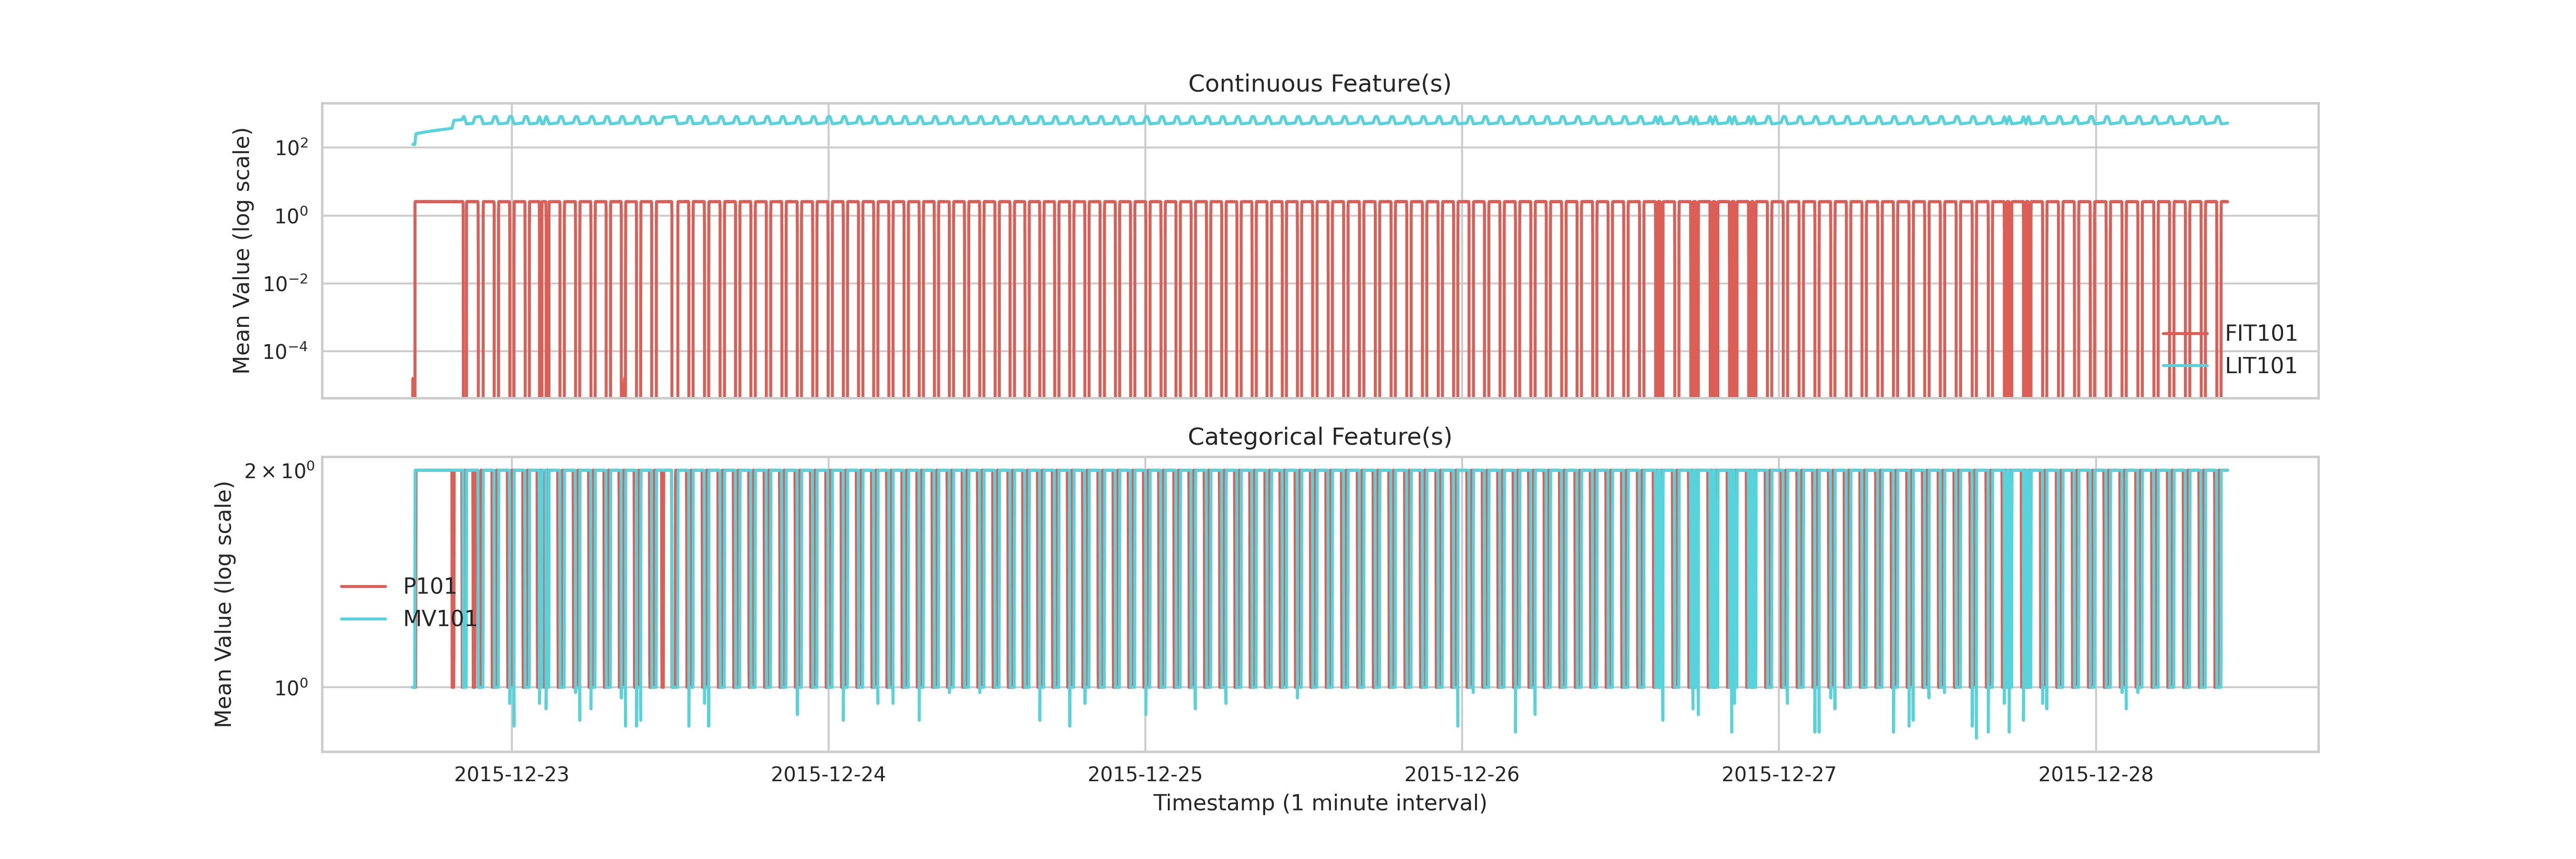
\includegraphics[width=0.8\textwidth]{images/normal/normal_sub-system_1_1_min.png}
        \caption{$P_1$ Sub-system data (log scale), aggregated in 1-minute interval}
        \label{fig:normal-P1}            

        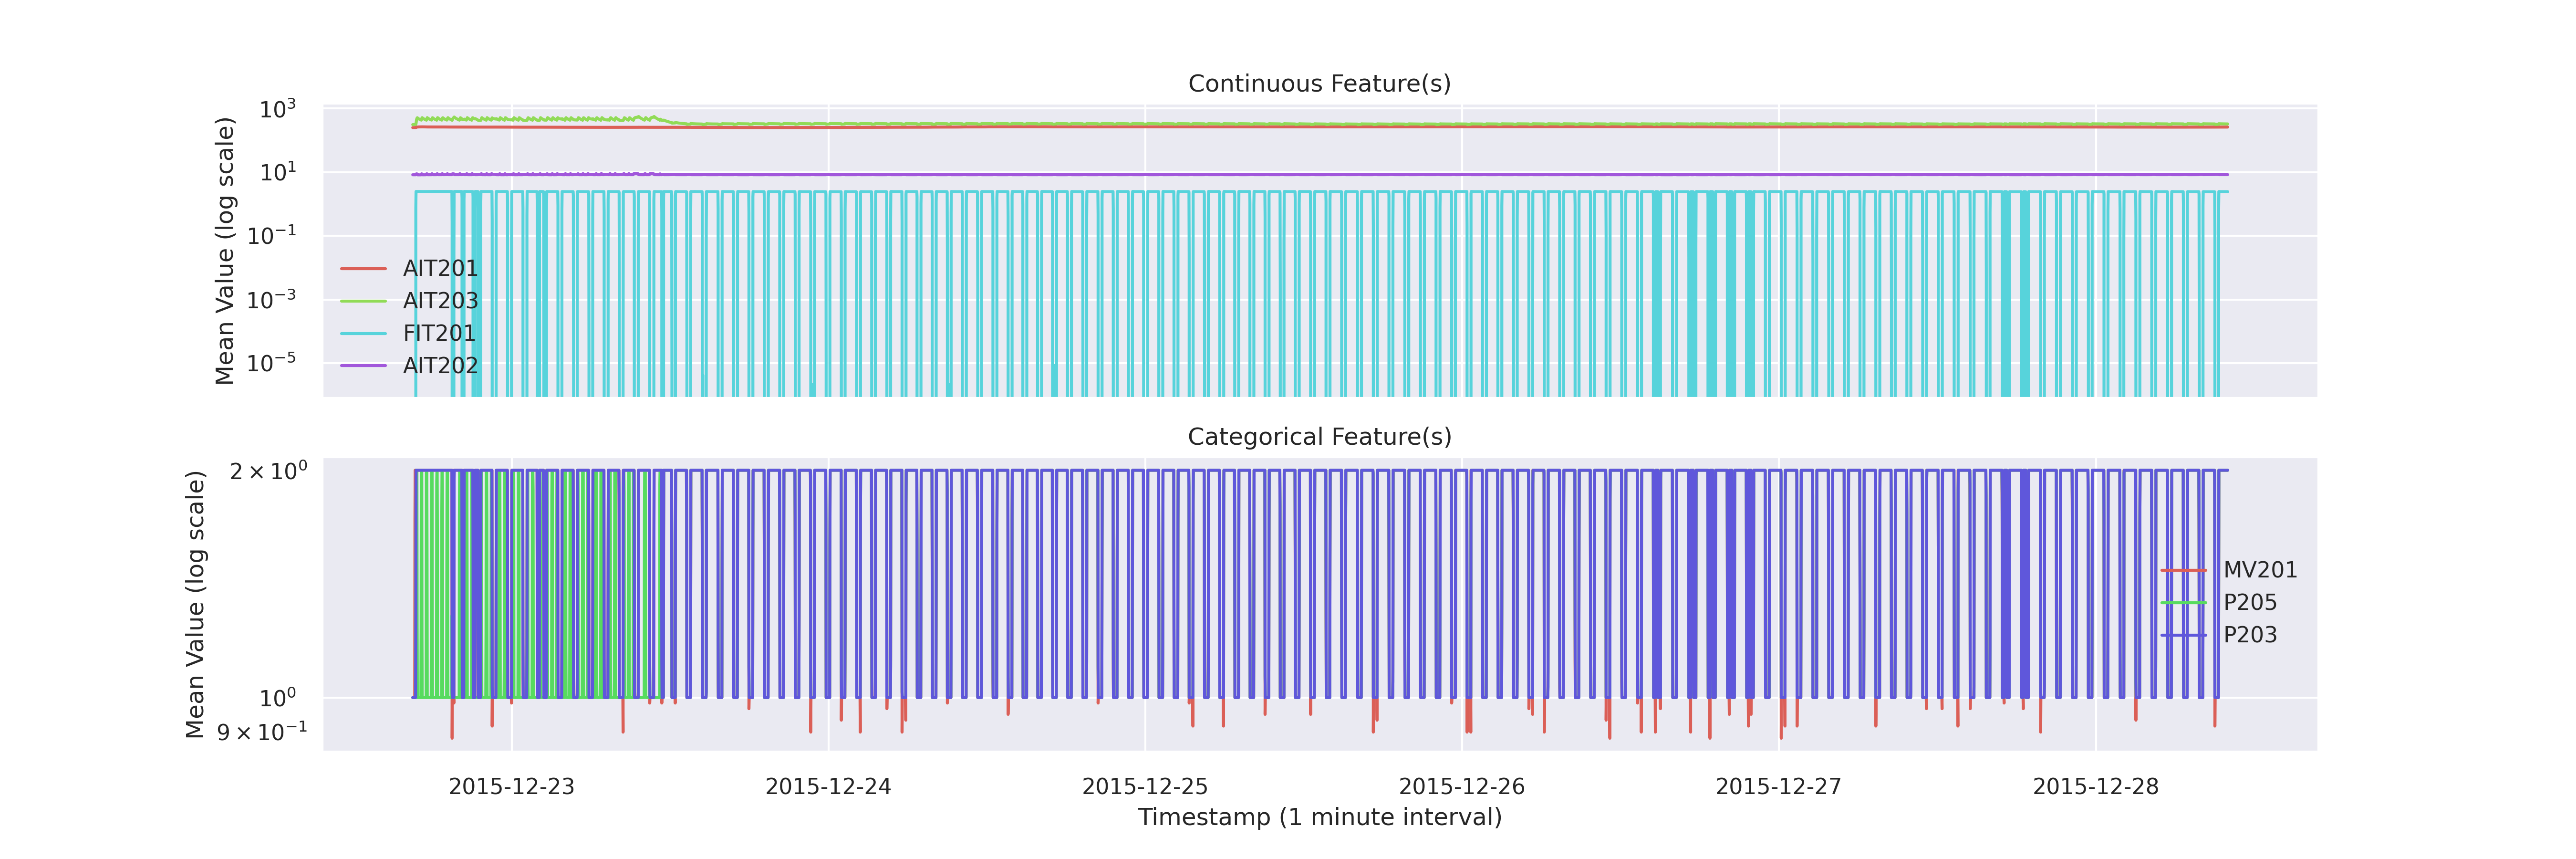
\includegraphics[width=0.9\textwidth]{images/normal/normal_sub-system_2_1_min.png}
        \caption{$P_2$ Sub-system data (log scale), aggregated in 1-minute interval}
        \label{fig:normal-P2}

        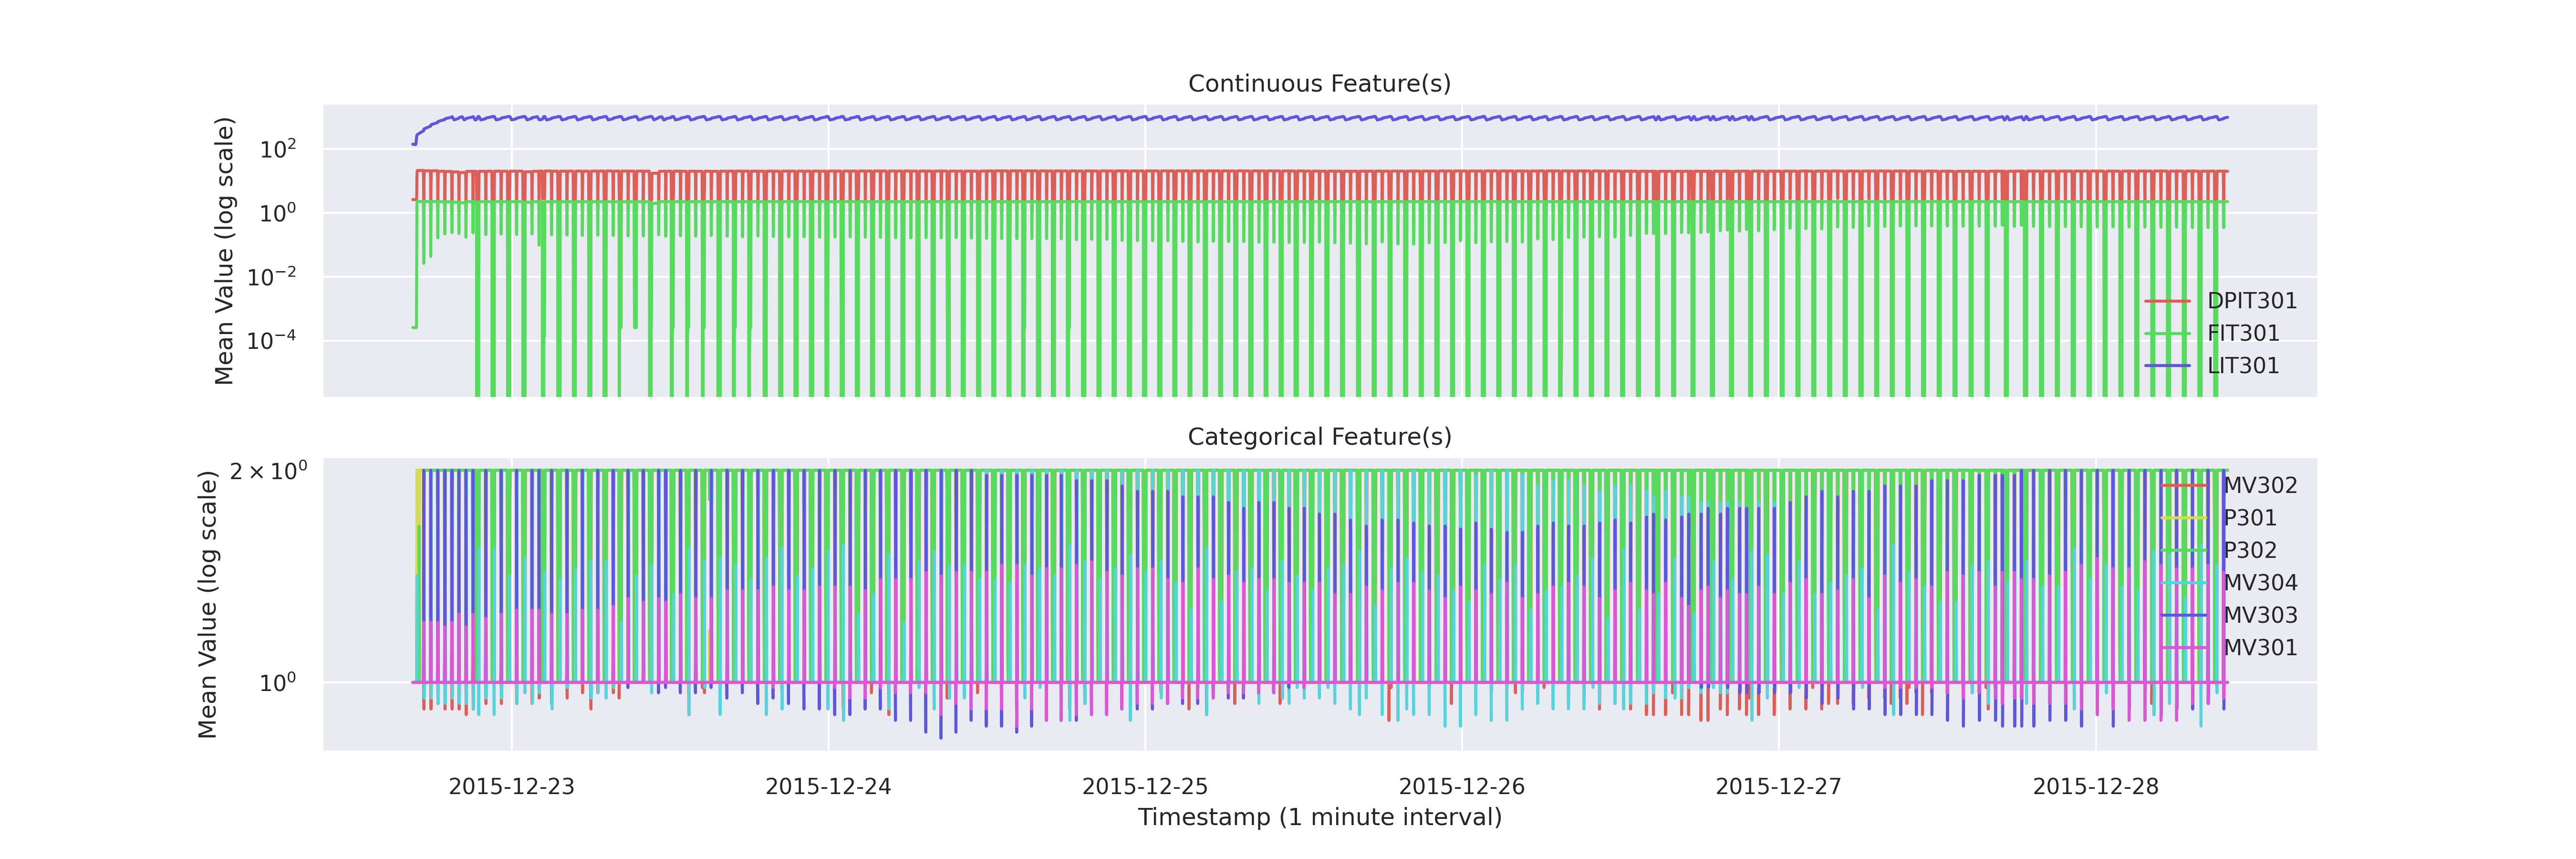
\includegraphics[width=0.9\textwidth]{images/normal/normal_sub-system_3_1_min.png}
        \caption{$P_3$ Sub-system data (log scale), aggregated in 1-minute interval}
        \label{fig:normal-P3}
    \end{figure}
    \clearpage
    \begin{figure}[!ht]

        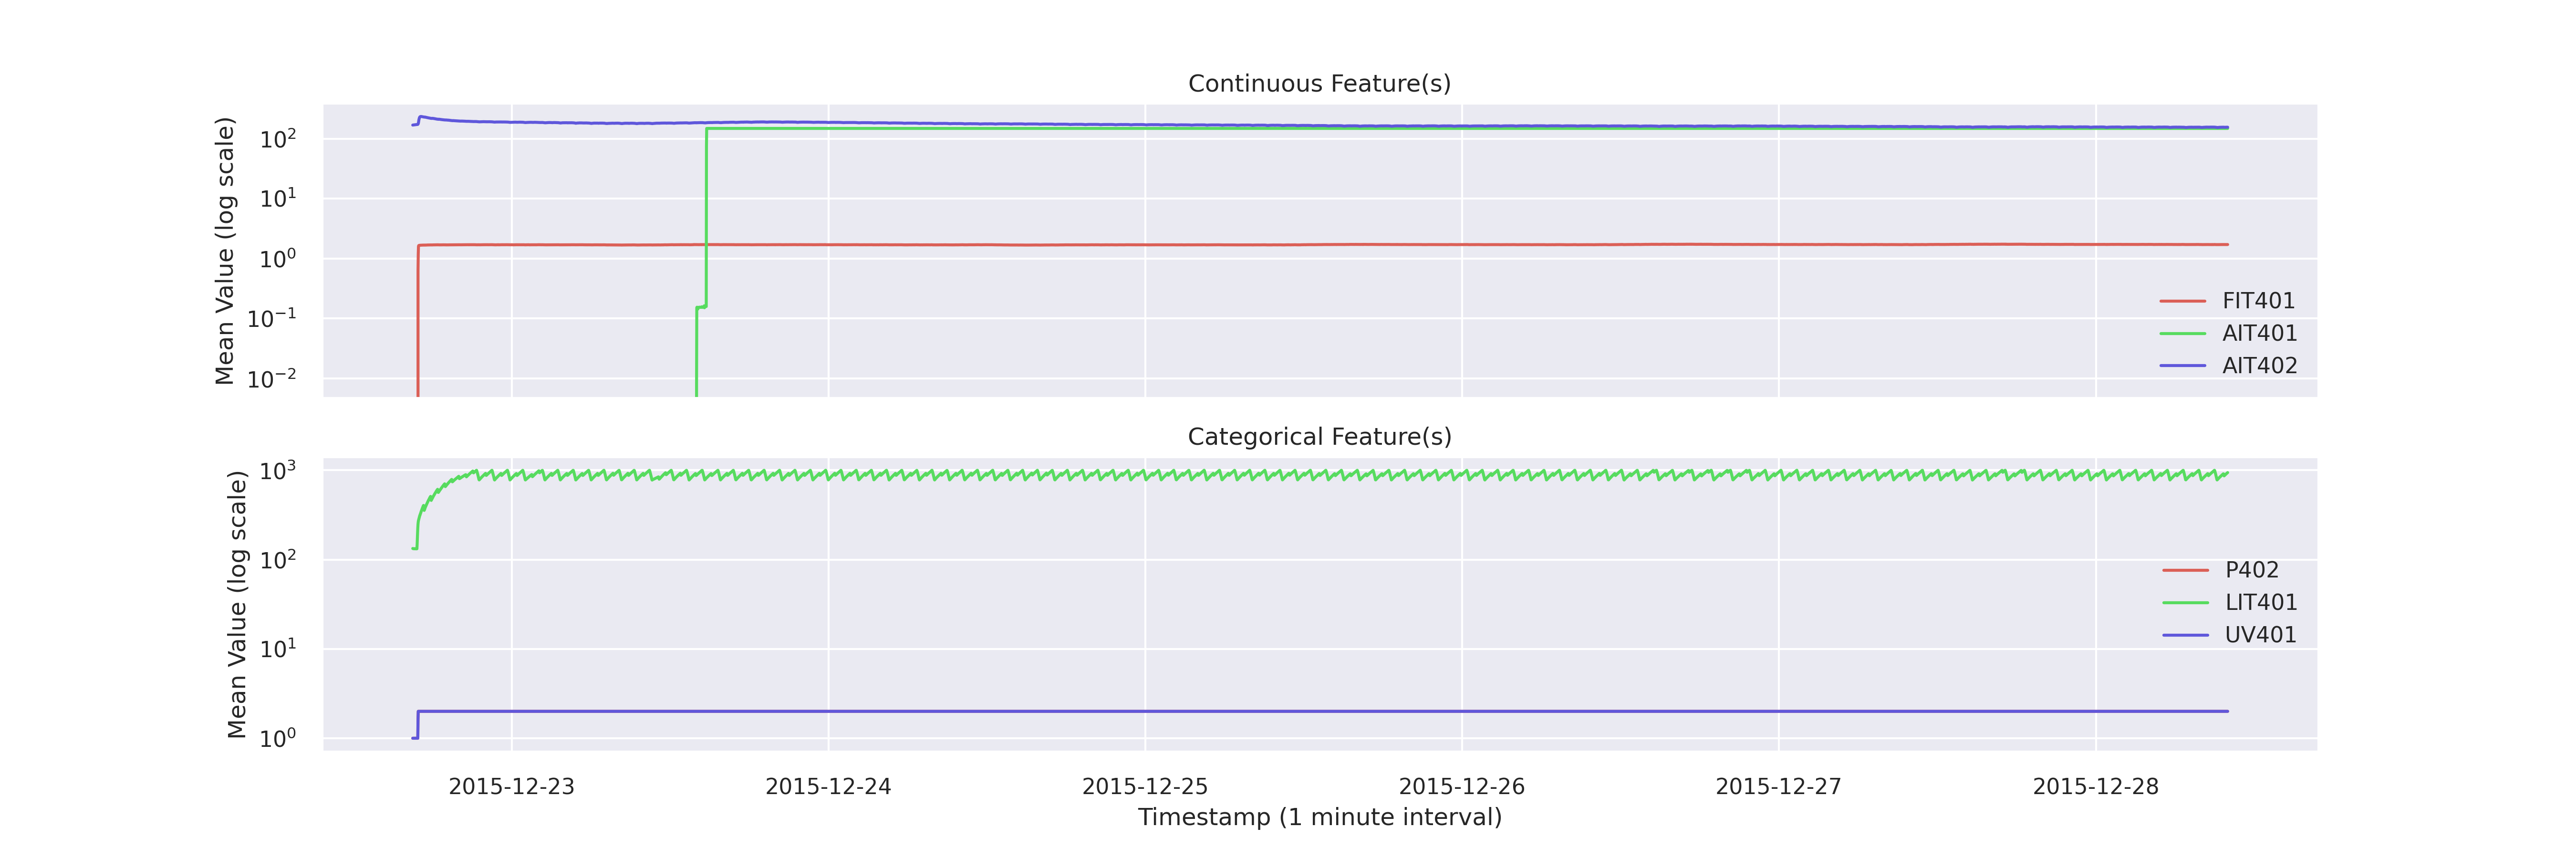
\includegraphics[width=0.9\textwidth]{images/normal/normal_sub-system_4_1_min.png}
        \caption{$P_4$ Sub-system data (log scale), aggregated in 1-minute interval}
        \label{fig:normal-P4}            
        
        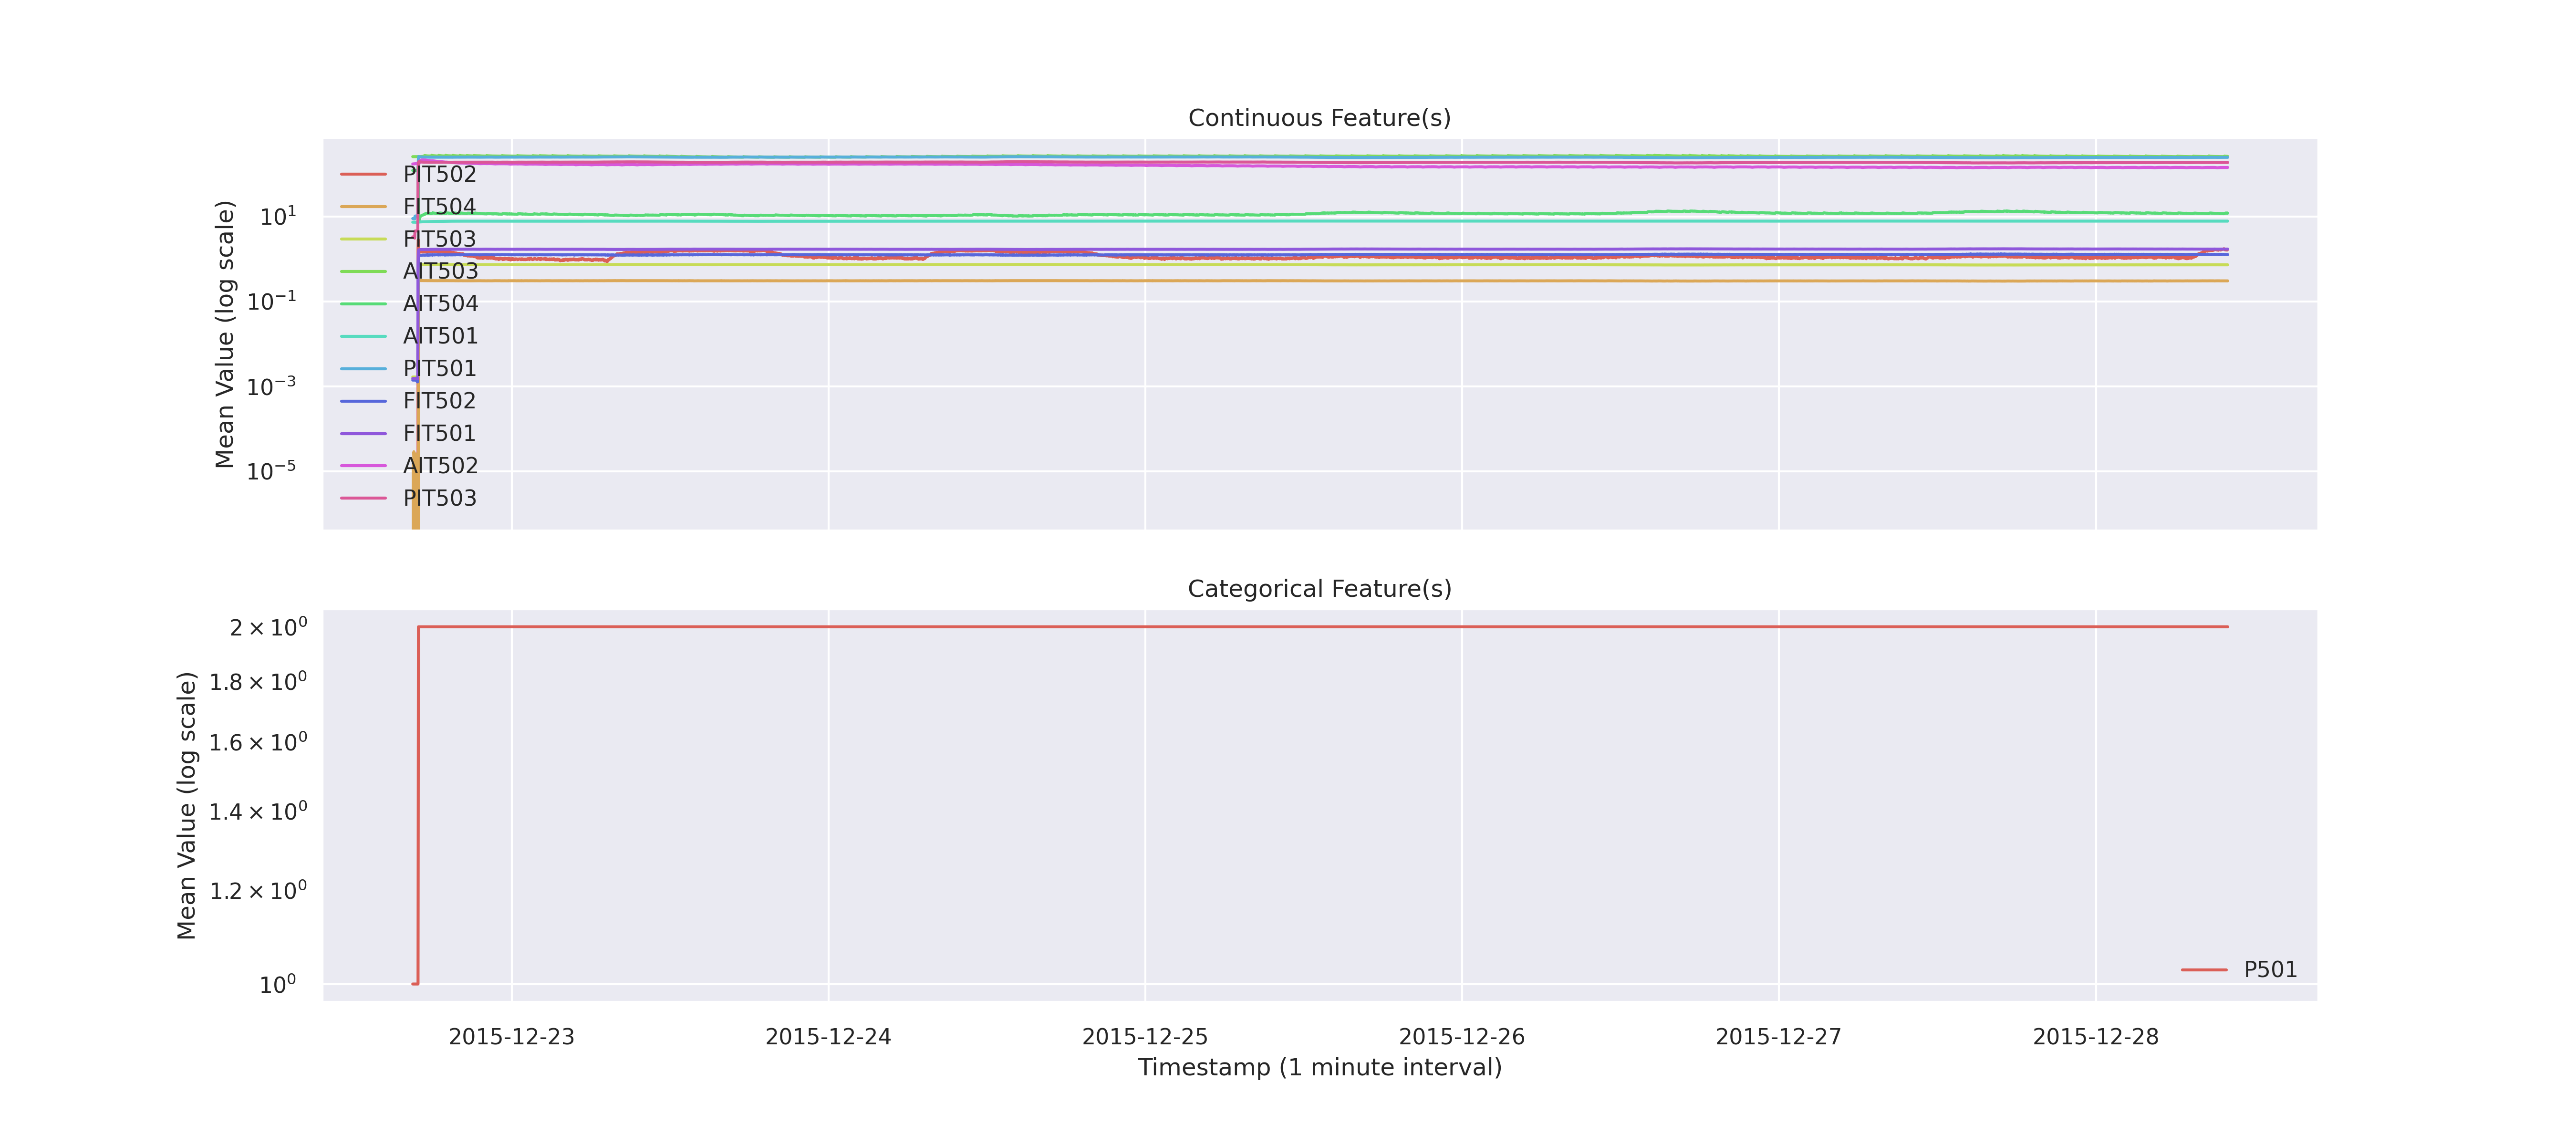
\includegraphics[width=0.9\textwidth]{images/normal/normal_sub-system_5_1_min.png}
        \caption{$P_5$ Sub-system data (log scale), aggregated in 1-minute interval}
        \label{fig:normal-P5}

        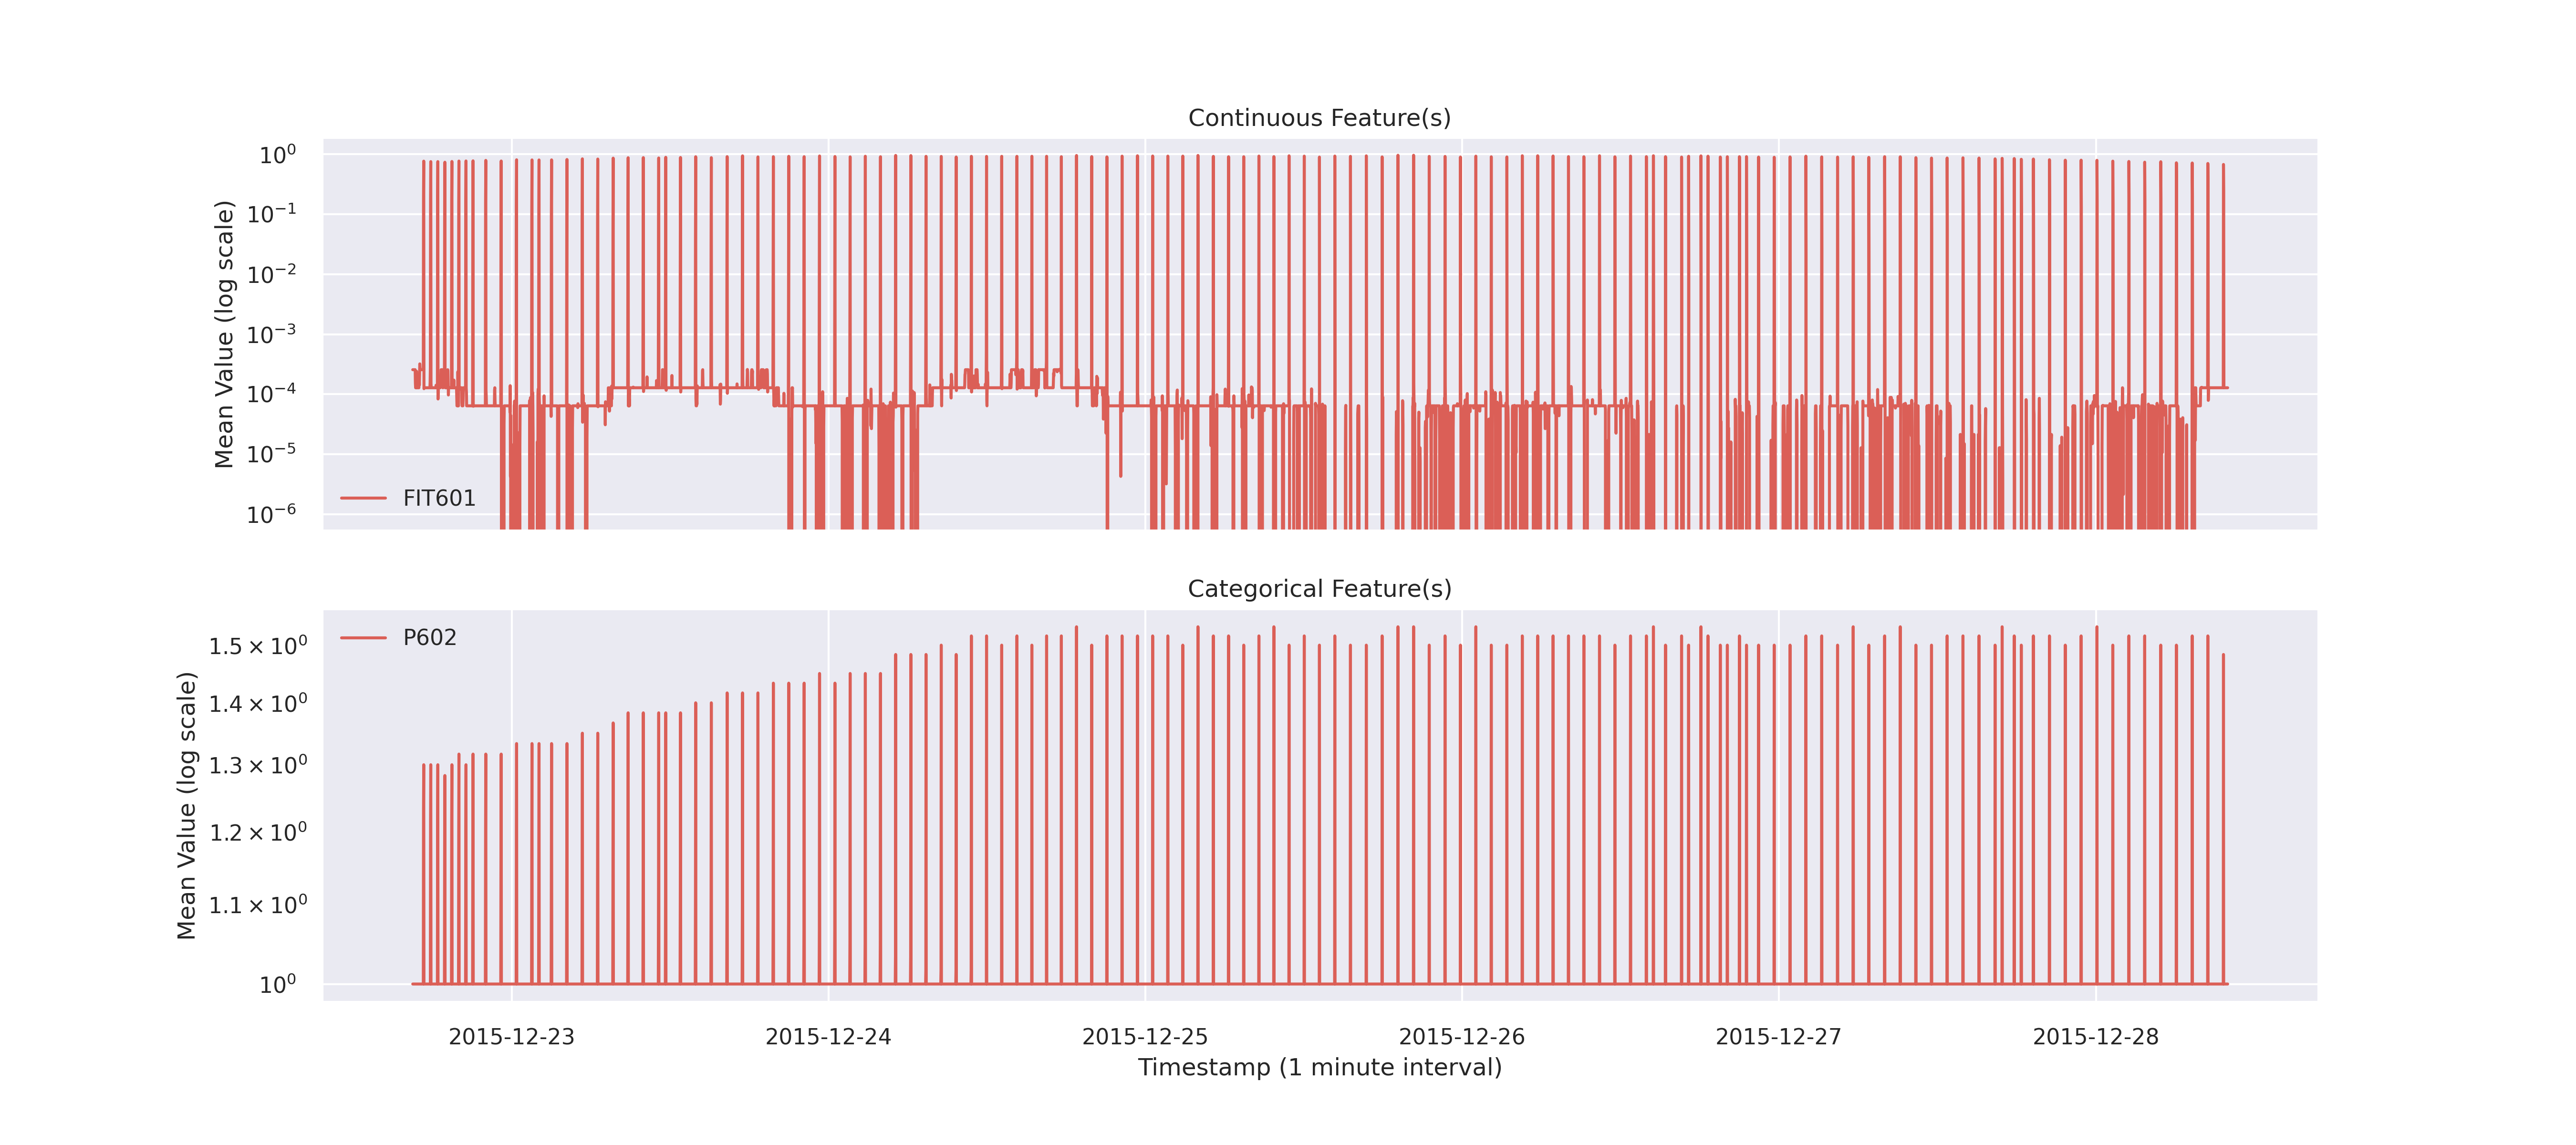
\includegraphics[width=0.9\textwidth]{images/normal/normal_sub-system_6_1_min.png}
        \caption{$P_6$ Sub-system data (log scale), aggregated in 1-minute interval}
        \label{fig:normal-P6}

    \end{figure}

\clearpage

\subsubsection{Visualize Attack Data by sub-systems}
    \begin{figure}[!ht]
        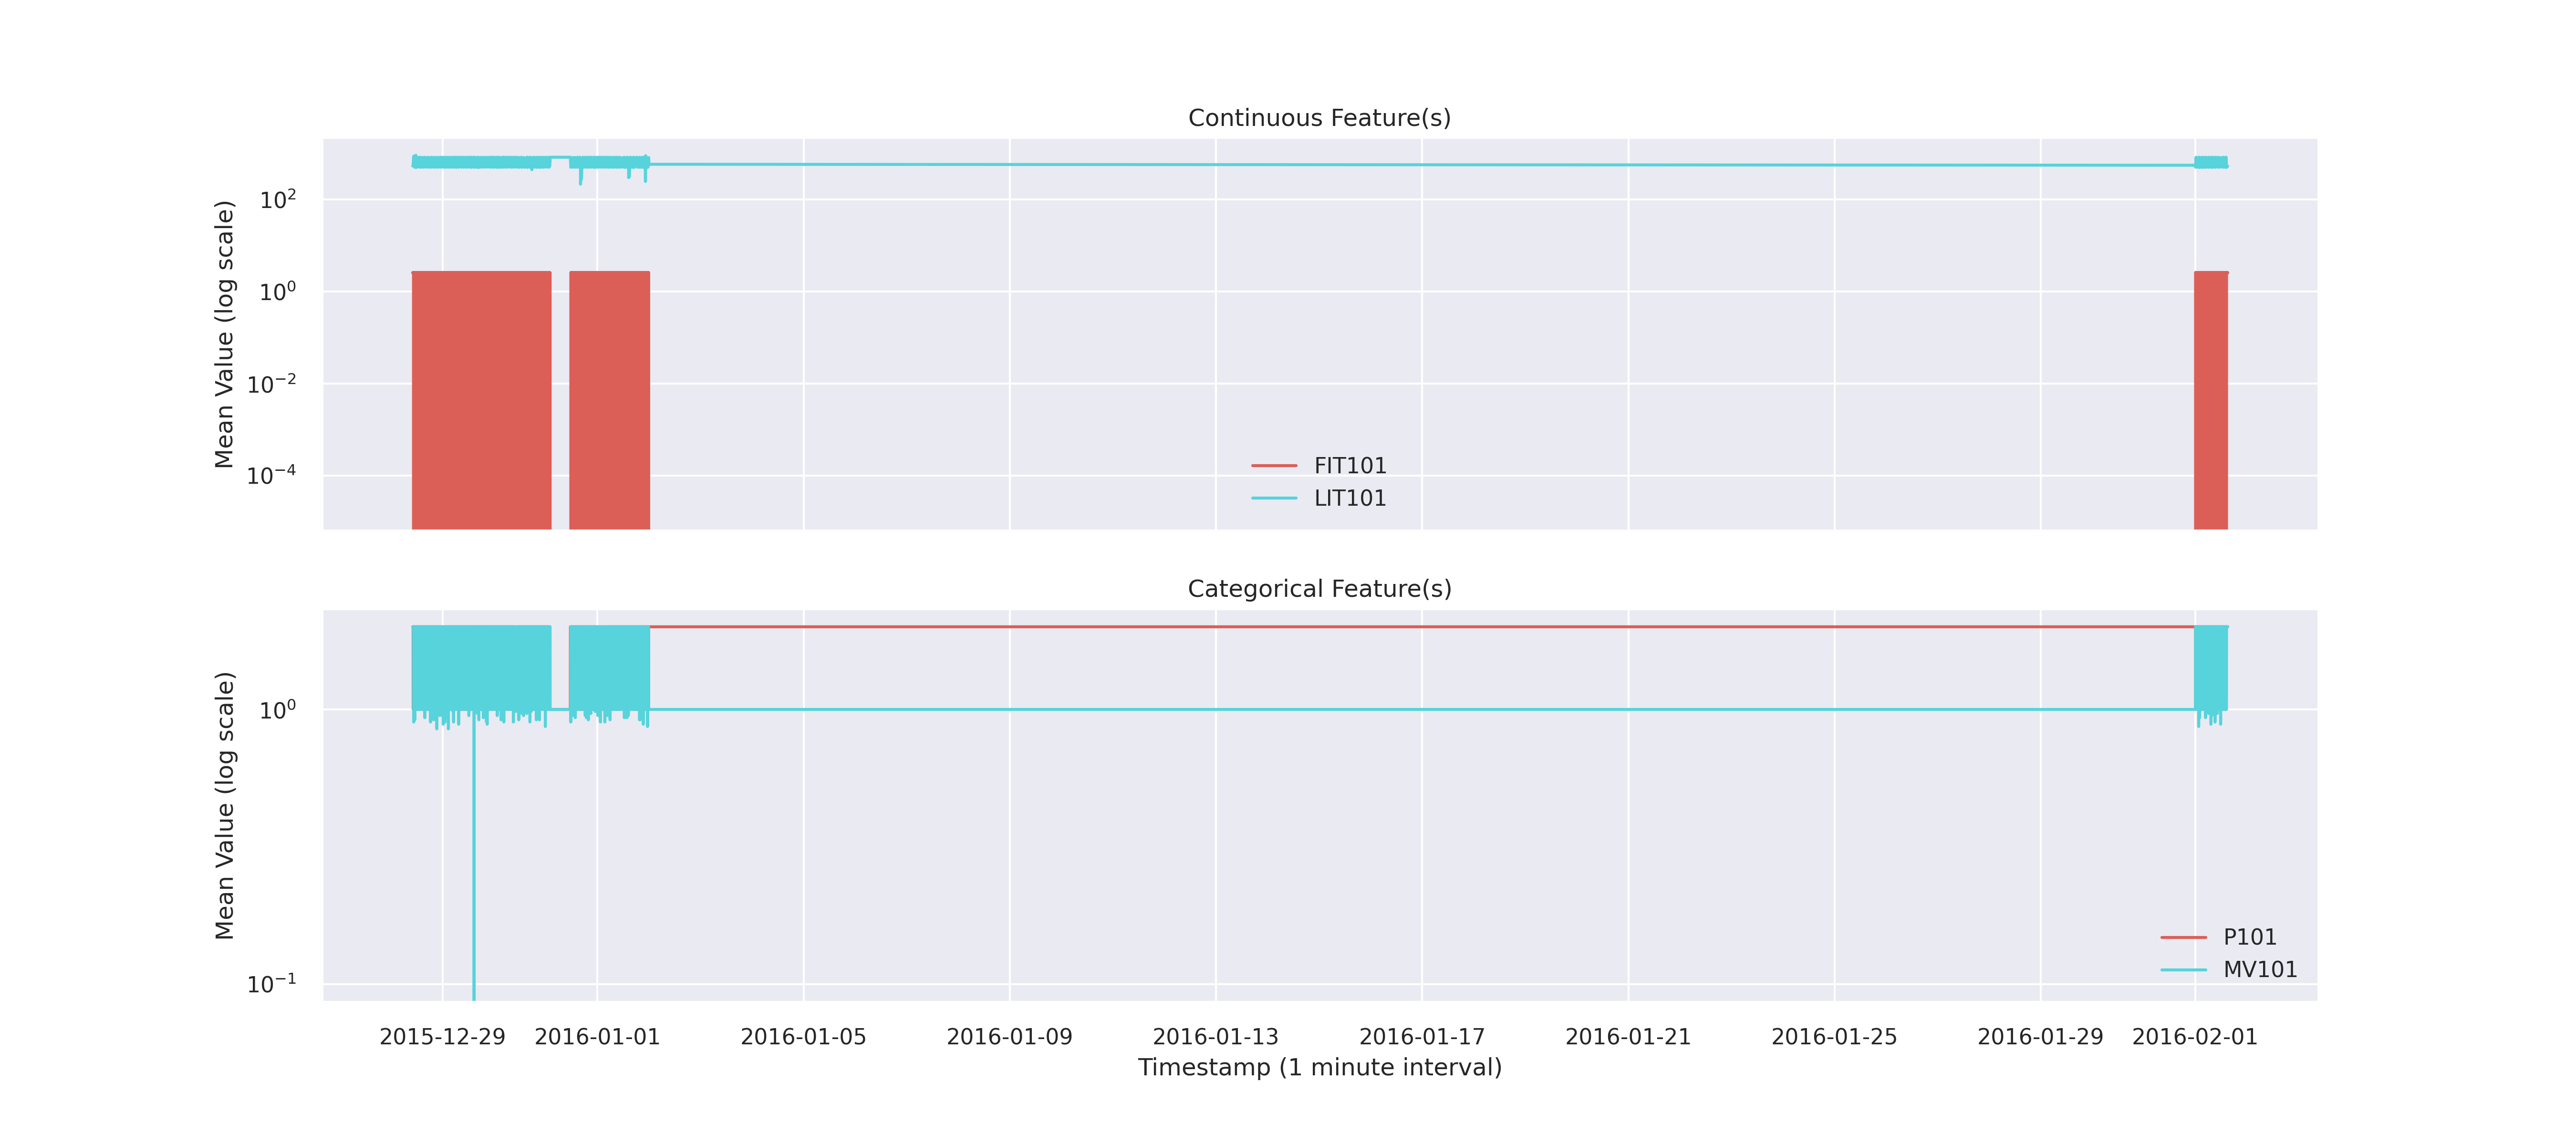
\includegraphics[width=0.9\textwidth]{images/attack/attack_sub-system_1_1_min.png}
        \caption{$P_1$ Sub-system data (log scale), aggregated in 1-minute interval}
        \label{fig:attack-P1}            

        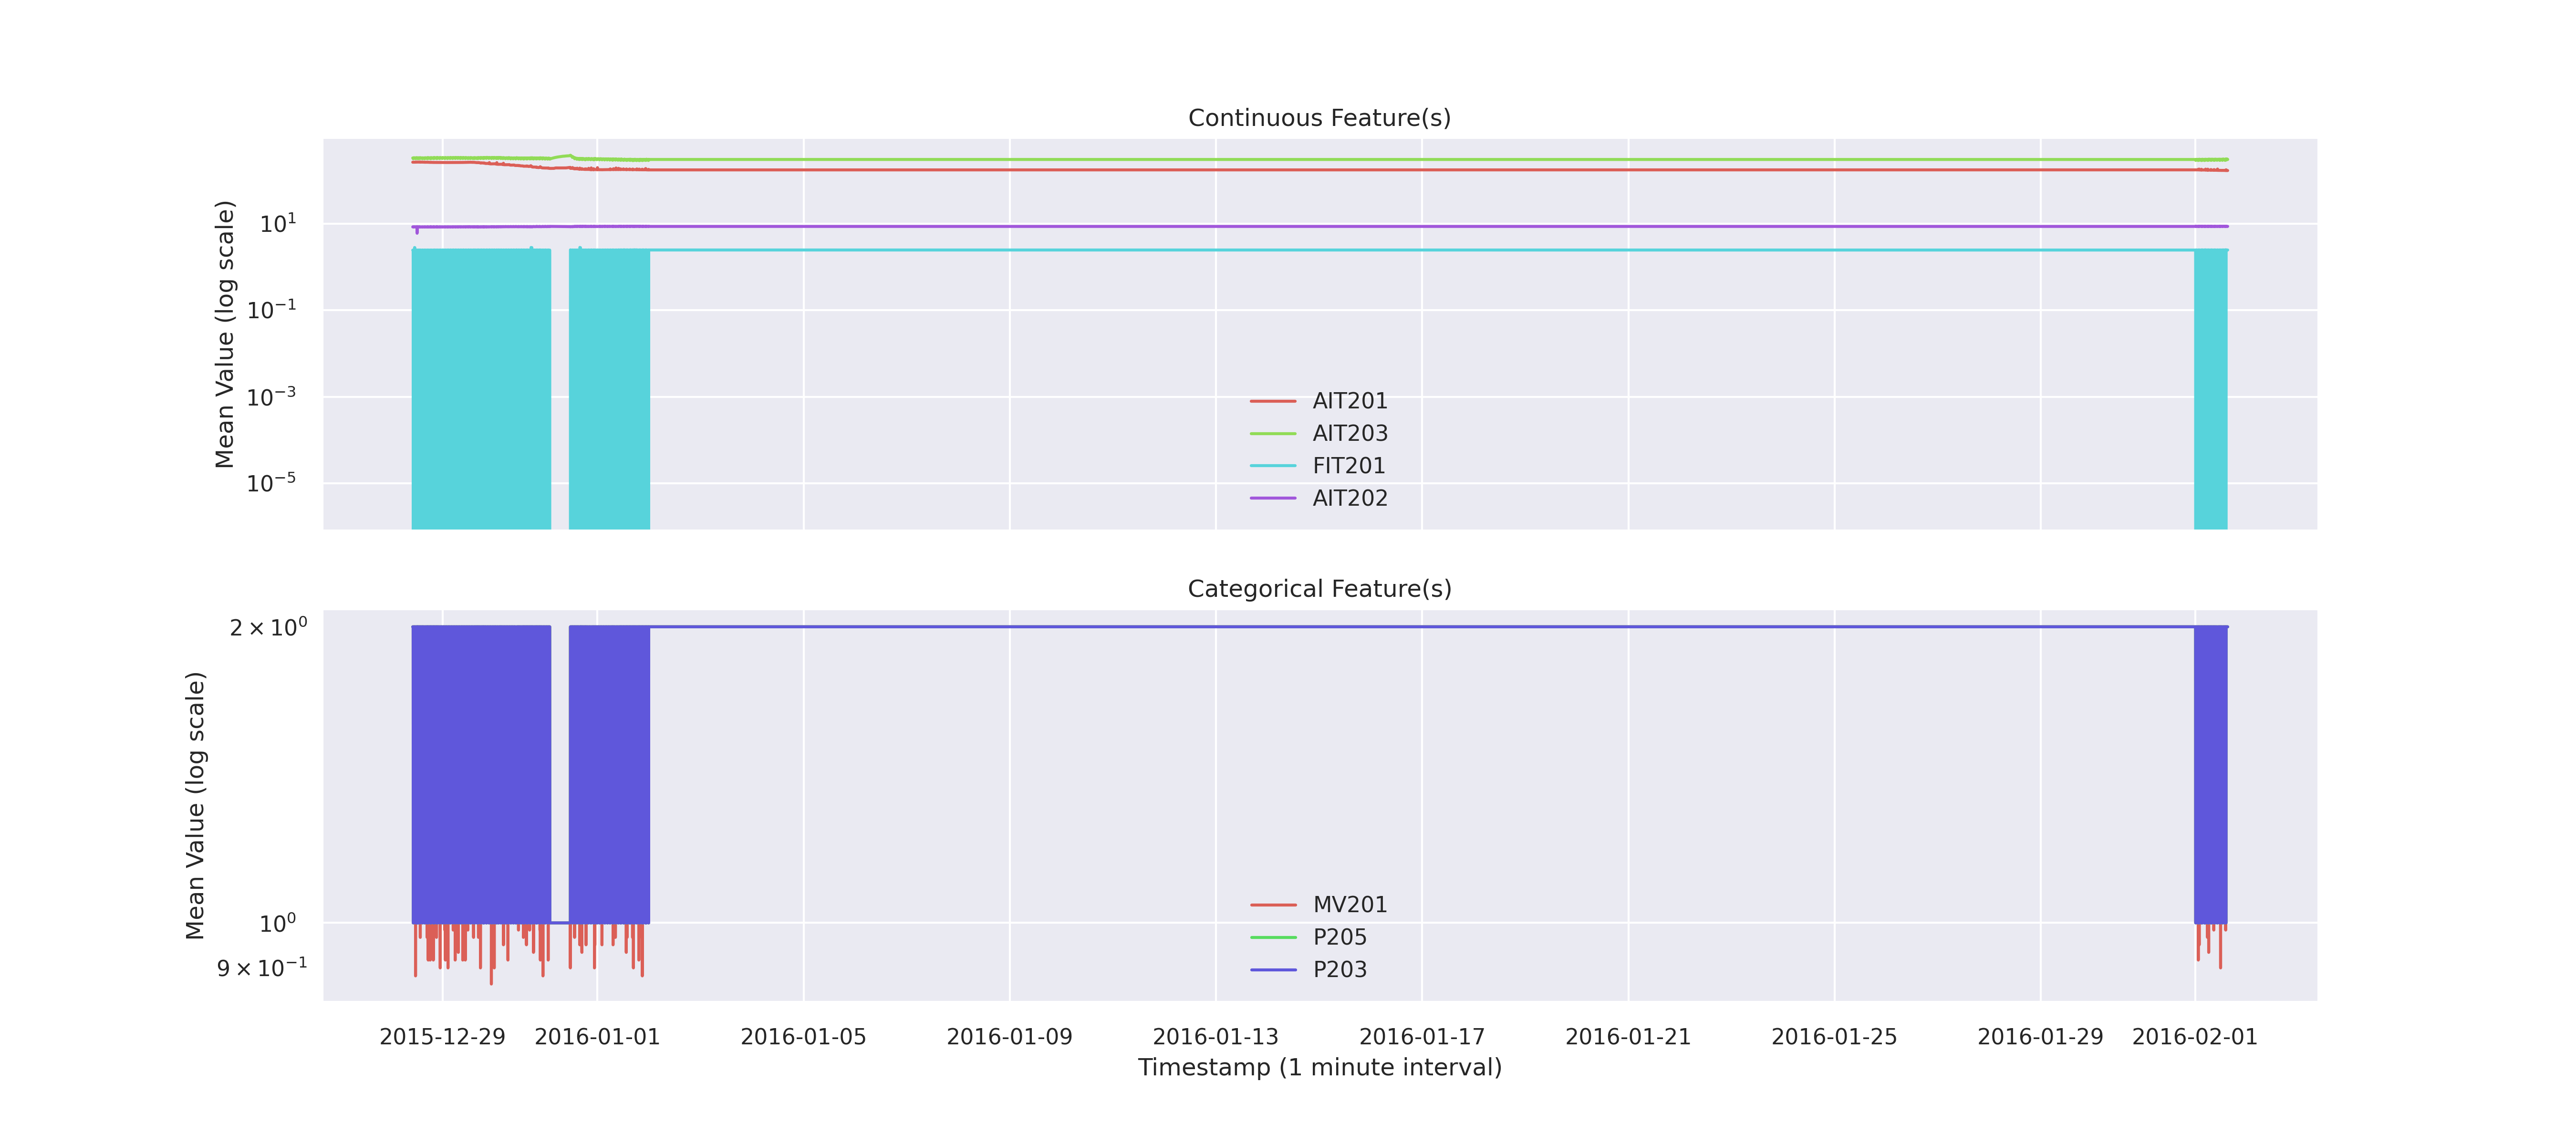
\includegraphics[width=0.9\textwidth]{images/attack/attack_sub-system_2_1_min.png}
        \caption{$P_2$ Sub-system data (log scale), aggregated in 1-minute interval}
        \label{fig:attack-P2}            

        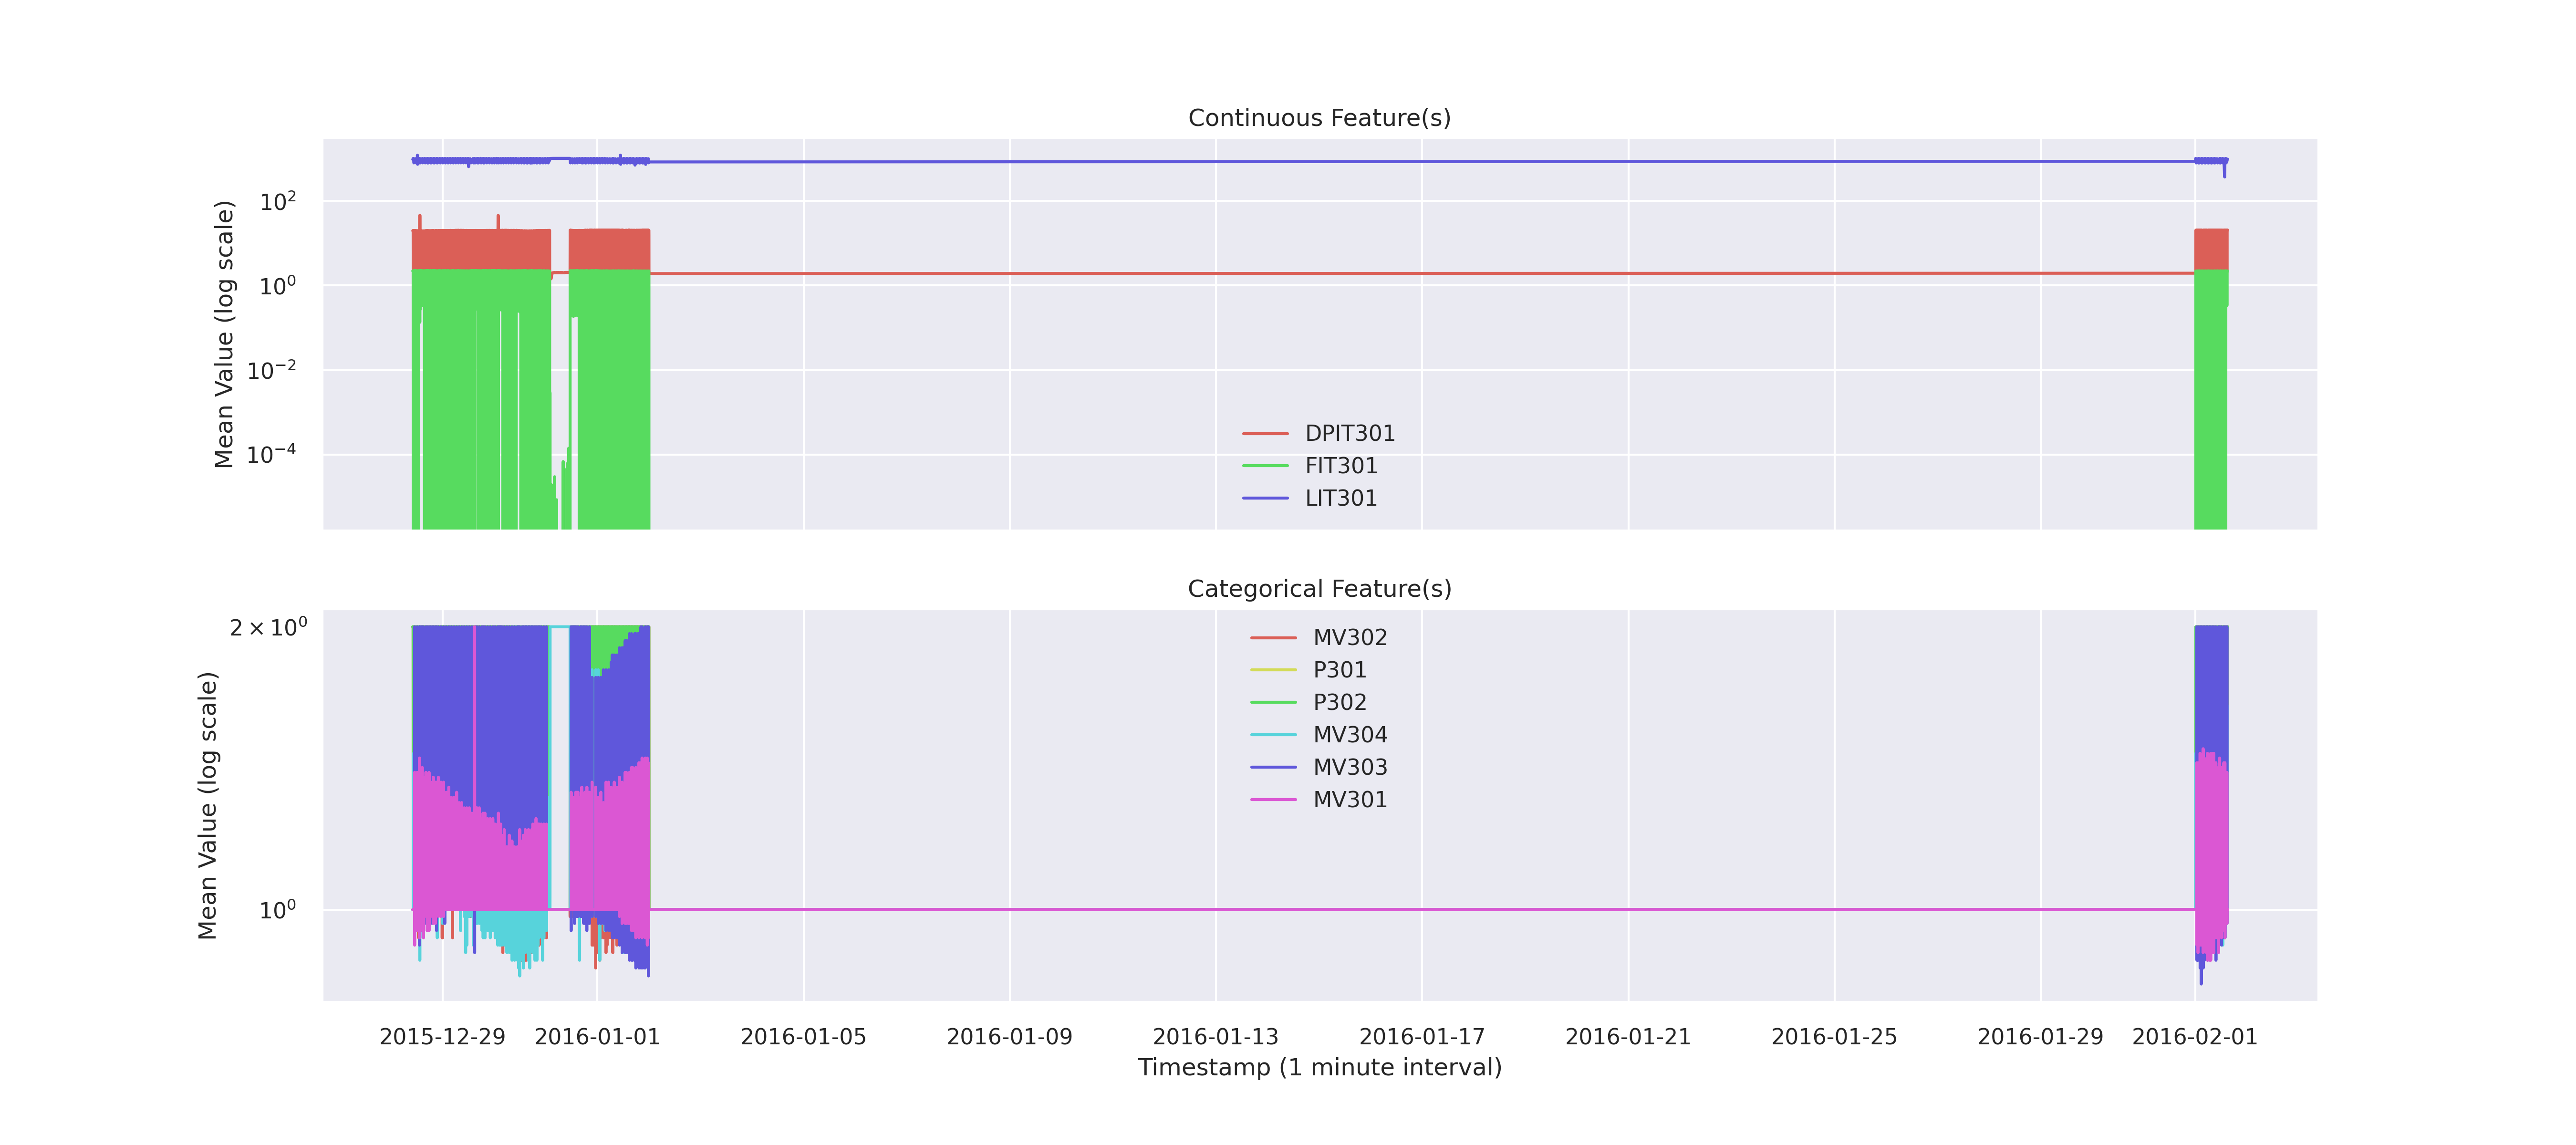
\includegraphics[width=0.9\textwidth]{images/attack/attack_sub-system_3_1_min.png}
        \caption{$P_3$ Sub-system data (log scale), aggregated in 1-minute interval}
        \label{fig:attack-P3}  
    \end{figure}
    \clearpage
    \begin{figure}[!ht]
        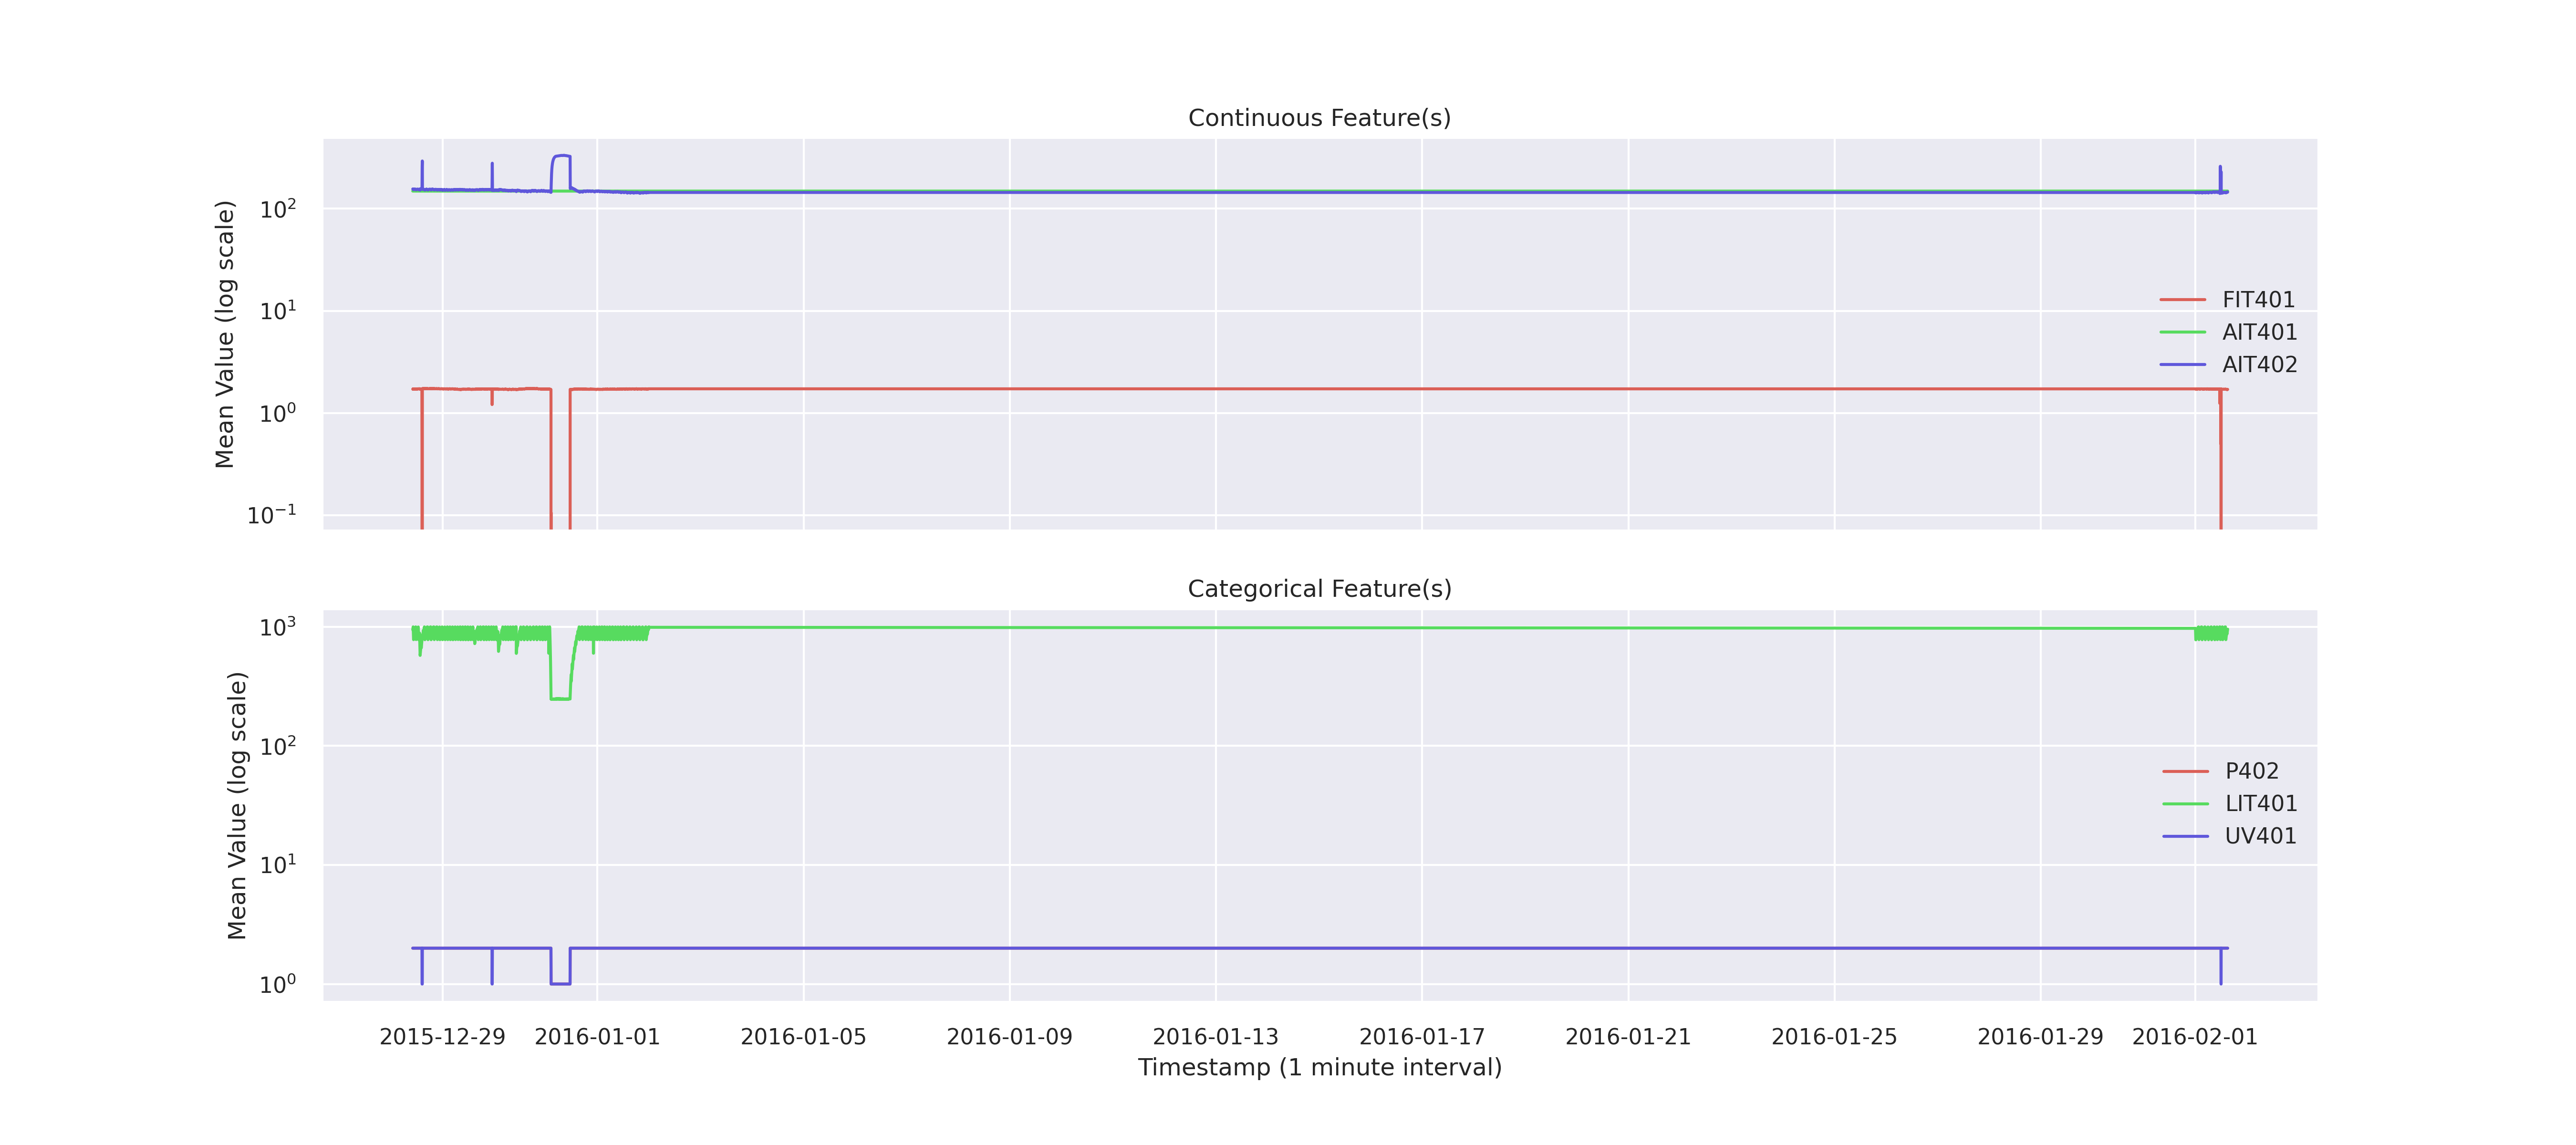
\includegraphics[width=0.9\textwidth]{images/attack/attack_sub-system_4_1_min.png}
        \caption{$P_4$ Sub-system data (log scale), aggregated in 1-minute interval. \\
        \textit{We can see anomalous behavior in Sensor and Actuator data $P_5$ sub-system on 01-Jan-2016.}}
        \label{fig:attack-P4}            

        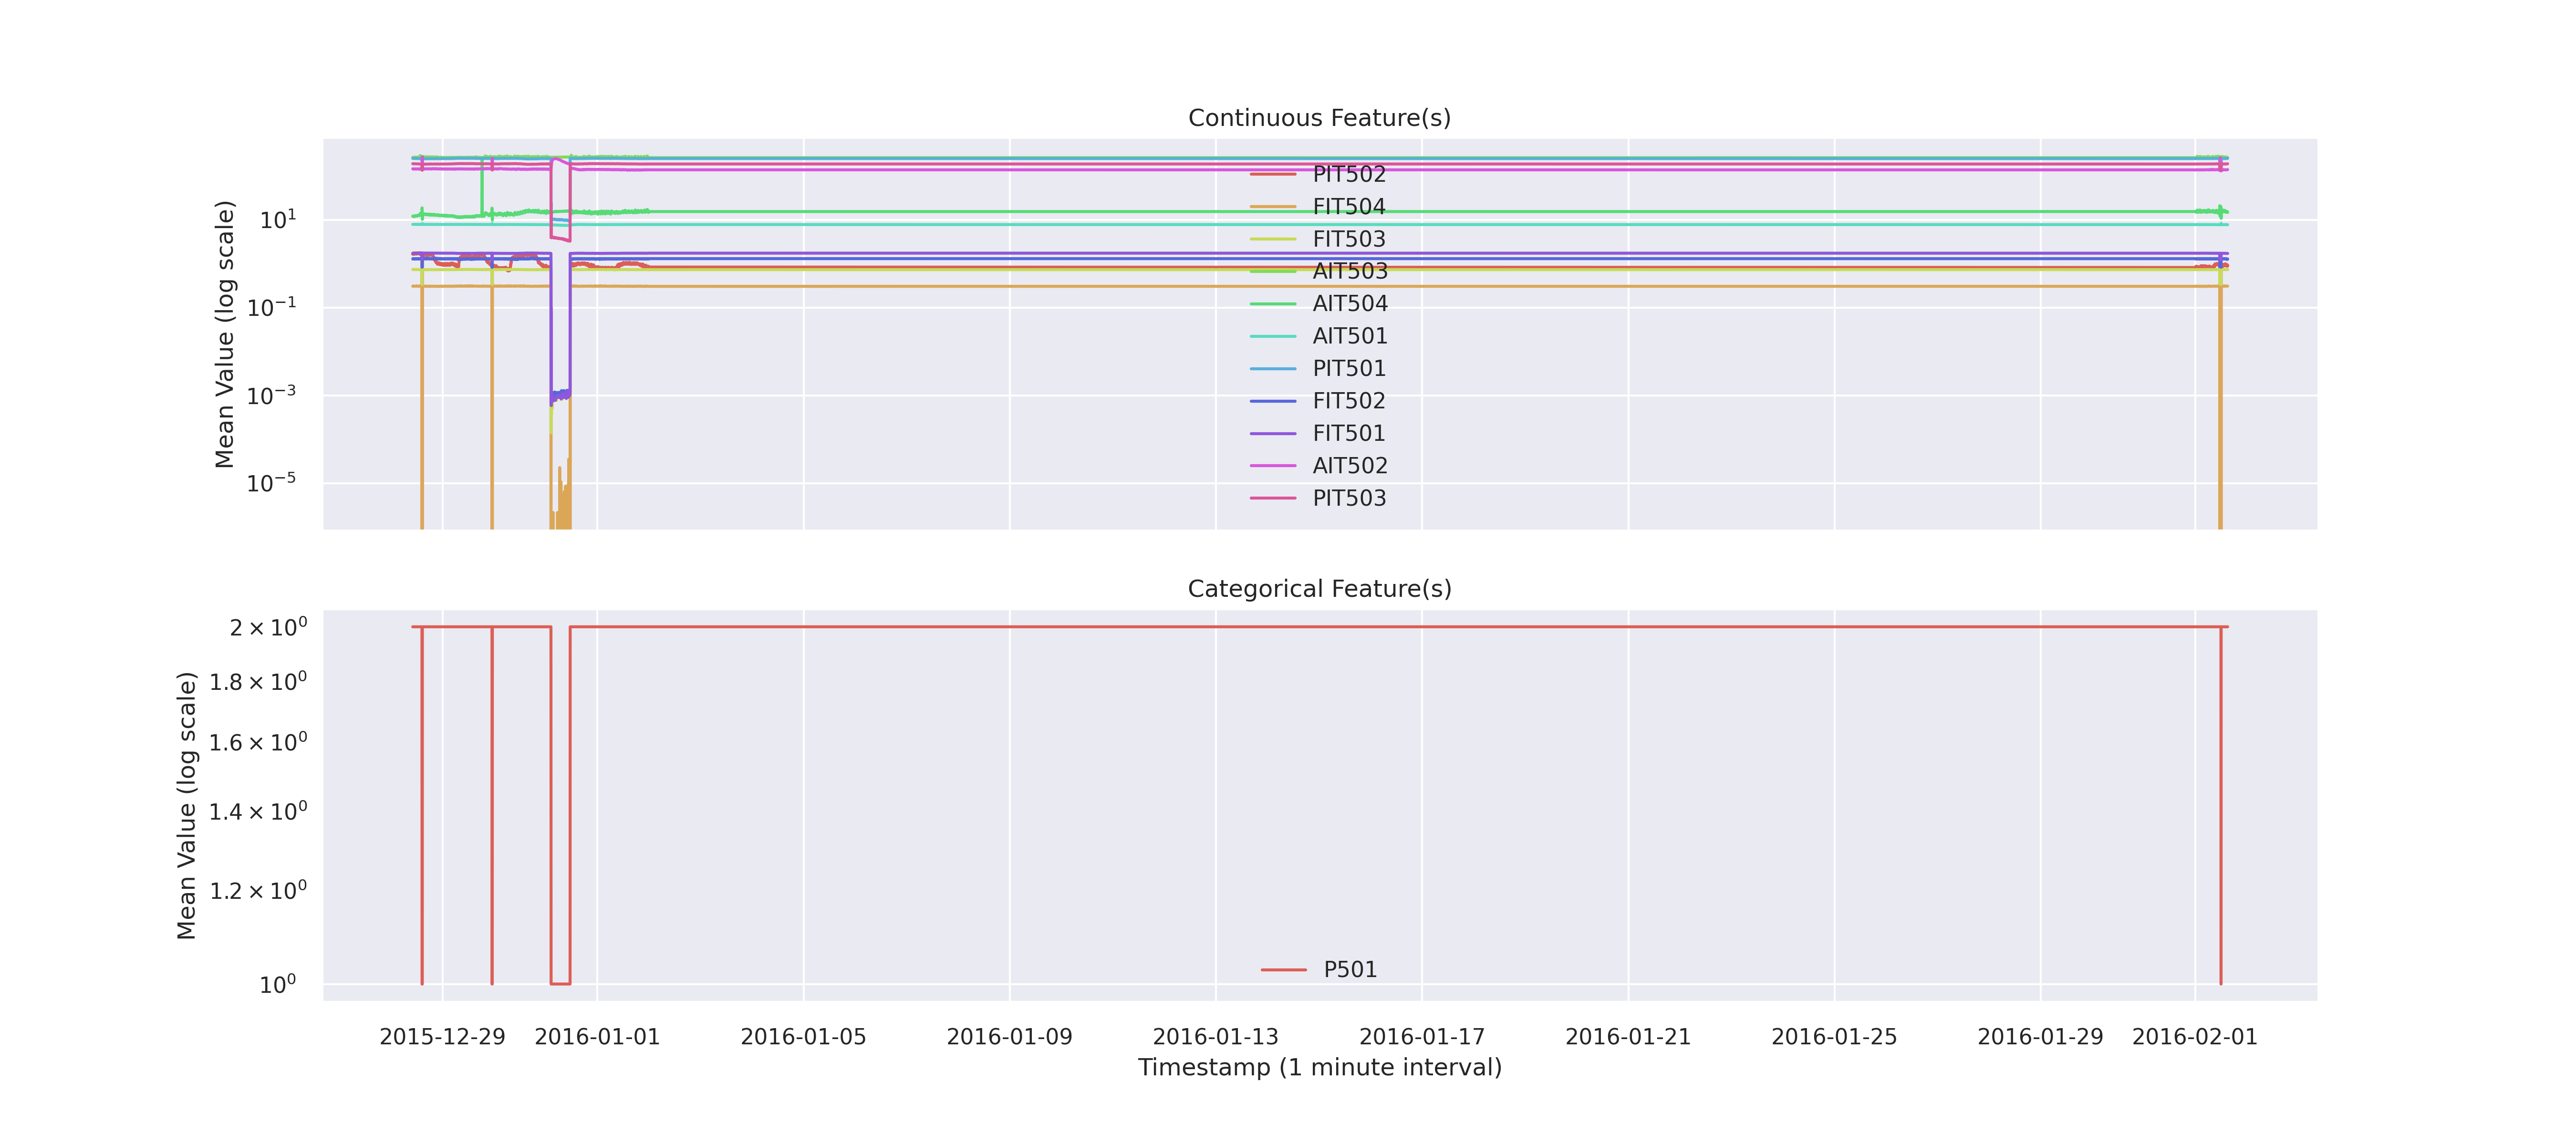
\includegraphics[width=0.9\textwidth]{images/attack/attack_sub-system_5_1_min.png}
        \caption{$P_5$ Sub-system data (log scale), aggregated in 1-minute interval. \\
        \textit{Similar to $P_4$, we can see anomalous behavior in Sensor and Actuator data $P_5$ sub-system on 01-Jan-2016.}}
        \label{fig:attack-P5}            

        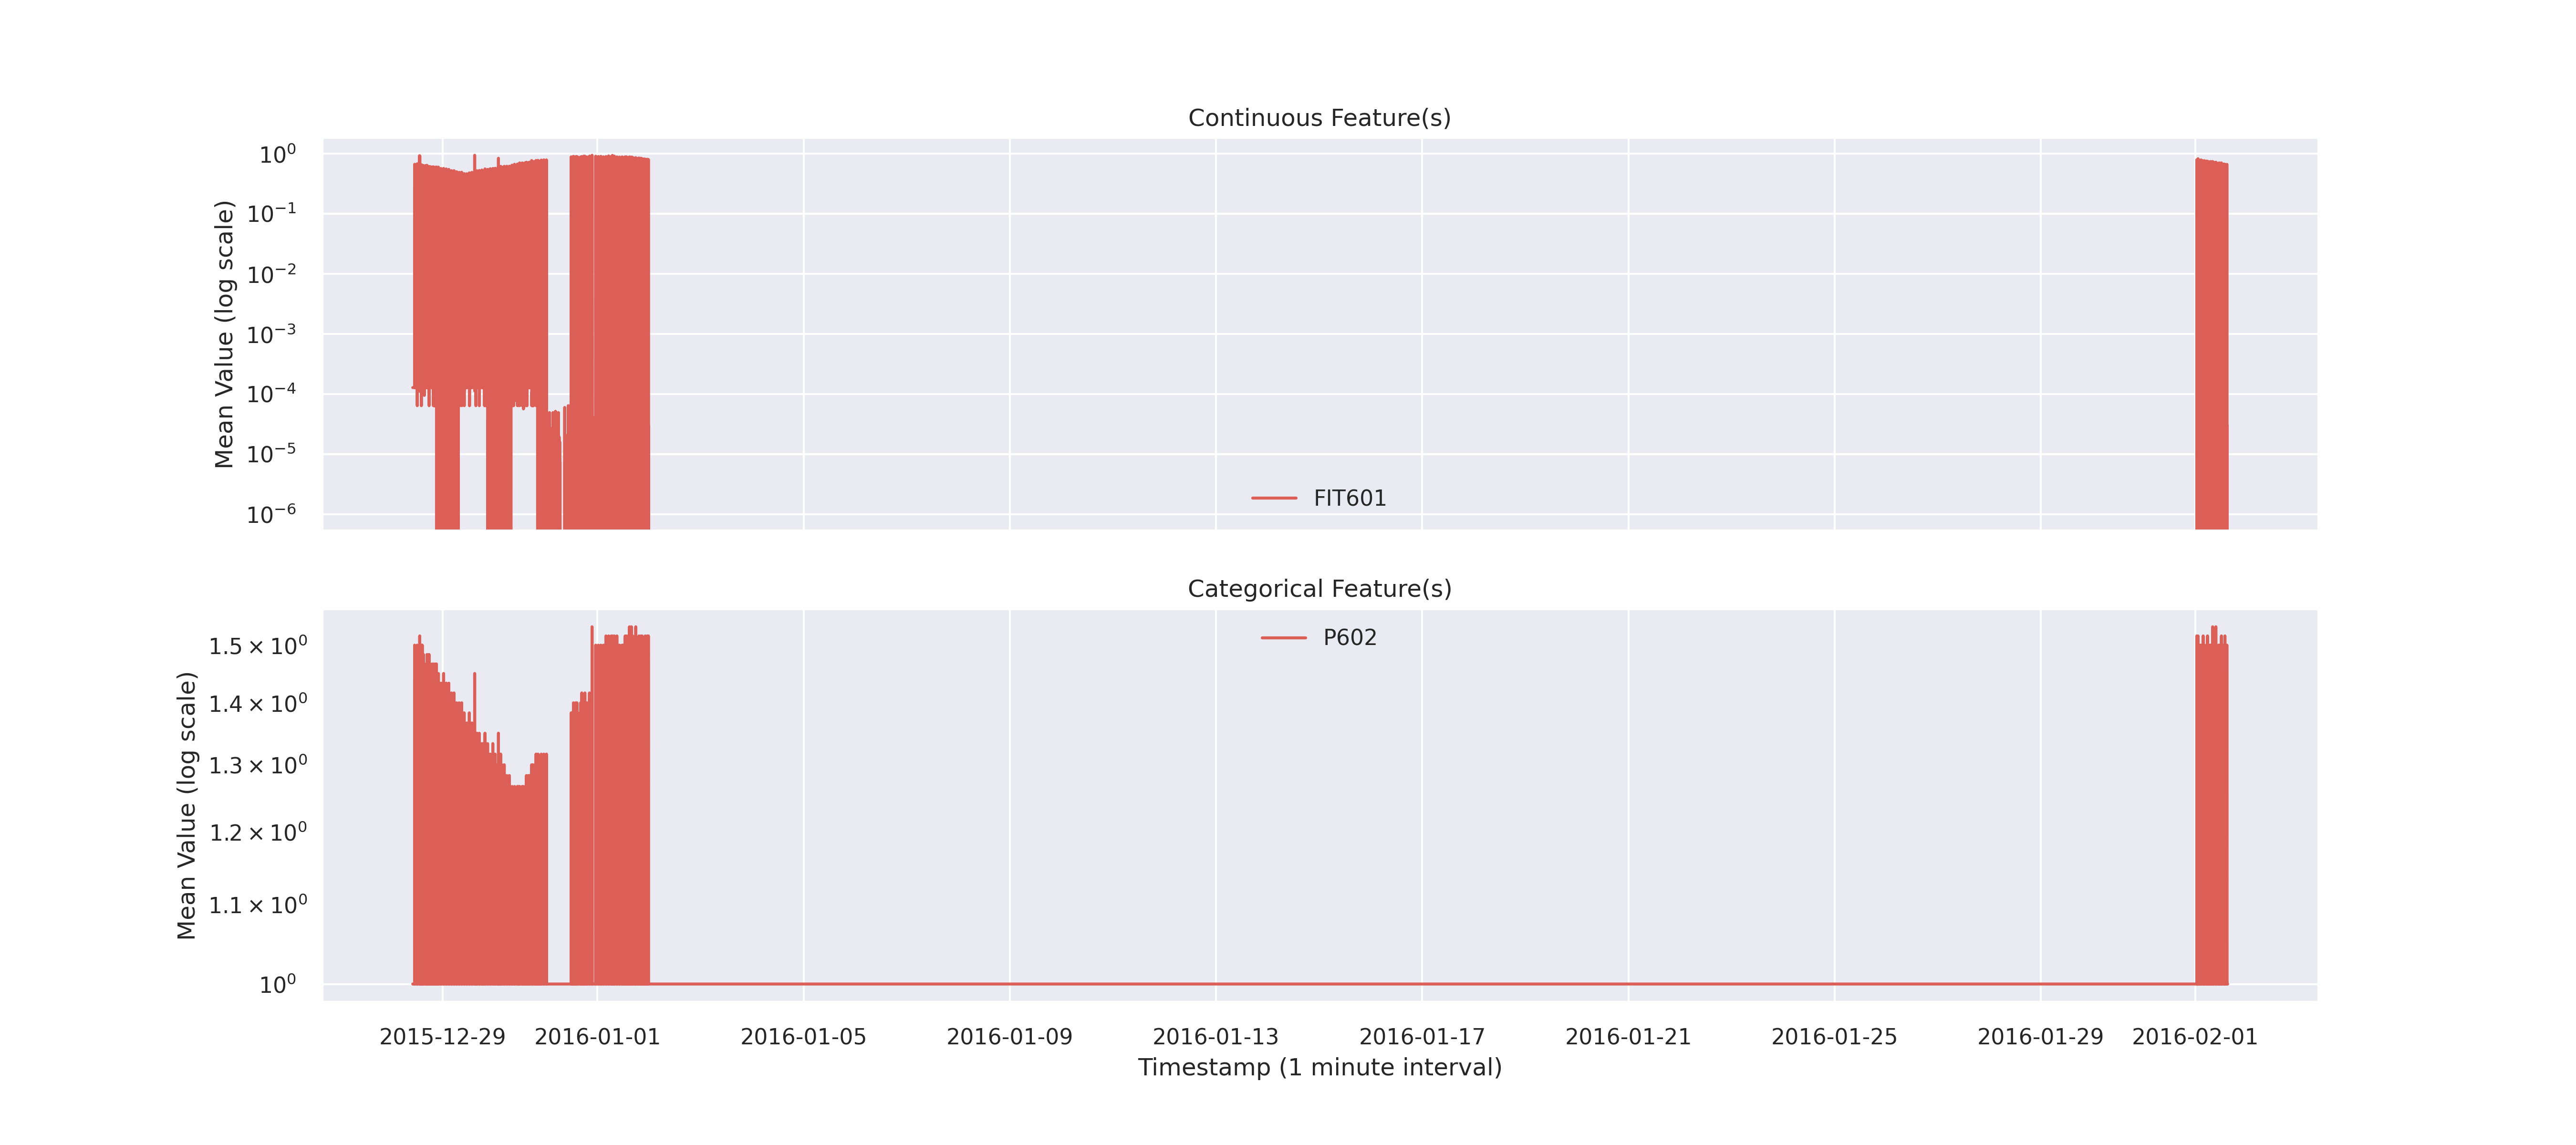
\includegraphics[width=0.9\textwidth]{images/attack/attack_sub-system_6_1_min.png}
        \caption{$P_6$ Sub-system data (log scale), aggregated in 1-minute interval}
        \label{fig:attack-P6}            
    \end{figure}

\clearpage
%TODO: KK - add heatmap and other analysis images here (Provide minimal textual description for each image) --> Done
%TODO: KK - add feature distribution graph --> Done
% TODO: Sumit: Add data distribution images here. Provide minimal textual description for each image). - Done
%TODO: Create github / google drive folders and use the link. KK to send email and get confirmation. --> Sent email; We need to send Git Repo; We will put all the images in report (As Annexure) There is no page limit - as such - based on Slack thread
%TODO: Mention about pickling. - Assigned to Sumit : Mention this in README.md
%TODO: Sumit: Feature selection: Mention Sub-system wise features - Done
%TODO: Sumit: Mention that reduce dataframe size by data type conversion (Float64 -> float32 and int64 -> category) - NOT NEEDED
%TODO: Sumit: Please provide the plot for each of algorithm (from sklearn documentation)


\subsection{Feature selection} \label{featureSelection}
Almost all features required for the model are provided in the data. However, the following data-cleaning tasks are required in order to utilize the dataset: 
\begin{enumerate}
    \item Create valid data frames with headers and values
    \item Convert DateTime strings to Timestamp and sensor/actuator data values to numeric.
    \item Valid column names and values removing leading/trailing spaces    
\end{enumerate}
As part of feature engineering, each sub-system sensor/actuator data will be extracted as a feature for unsupervised learning. \\
We will also ignore the label data `Normal/Attack' as per recommendation.

\subsection{Develop Unsupervised Model}
To develop the model, we will take the following steps: 
\begin{enumerate}
    \item We will train the model for each of the Sub-systems separately. This decision was taken due to memory/infrastructure constraints for training the full model with all records and features. We assume that each of the sub-systems is independent and hence it will not bias the model's predictions. We validated this assumption with Project sponsors. 
    \item Merge non-anomalous and anomalous data while creating a `class` feature.
    \item Ensure that all data points either exhibit Gaussian (Normal) Distribution, or that they are transformed such that their distribution is normal. This is an important step before applying any probability-based learning algorithm.  
    \item Split the data into Training, Cross Validation (CV), and Test. However, the Training set will consist of completely non-anomalous data, whereas CV and Test datasets will distribute anomalous data 50\% each.
    \item Implement Unsupervised algorithm that computes Local Outlier Factor (LOF)\cite{three} using Mahalanobis Distance. LOF is an anomaly score computed for each sample. The locality is defined in terms of k-nearest neighbors using some distance measure. Mahalanobis works better with higher dimensional data.    
\end{enumerate}

\subsection{Model validation}
We trained the models on first 8 days of SWaT: \textsf{22-Dec-2015 to 28-Dec-2015 10:00 AM}. And tested  it against data from \textsf{28-Dec-2015 to 02-Jan-2016}. 

\section{Algorithm Description}
There are subtle differences between Outlier Detection and Novelty detection \cite{twelve}. Outliers are essentially observations that significantly
deviate from all other observations in a given training data. They can be treated as contamination and are generally discarded before using the training dataset. 
On the other hand, Novelty detection attempts to figure out if a new/unseen observation has a similar distribution as the training data. If the distributions do not match, we declare the new observation as an anomaly. 

There are various algorithms that help with detecting outliers as well as Novelties. We explored the below-listed algorithms on the provided dataset to come up with a robust anomaly detection model:
\begin{itemize}
    \item \textsf{Isolation Forest}
    \item \textsf{Minimum Covariance Determinant (MCD)}
    \item \textsf{One-Class Support Vector Machine (OCSVM)}
    \item \textsf{Local Outlier Factor (LOF)}
    \item \textsf{Histogram-Based Outlier}
    \item \textsf{K-nearest Neighbor (KNN)}    
\end{itemize}

\subsection{iforest}
An efficient way of performing outlier detection in high-dimensional datasets is to use random forests. The `iforest' \cite{five} algorithm `isolates' observations by randomly selecting a feature and then randomly selecting a split value between the maximum and minimum values of the selected feature. Recursive partitioning can be represented by a tree structure. The number of splittings required to isolate a sample is equivalent to the path length from the root node to the terminating node. \par 
Anomalies have a shorter path. Hence, when a forest of random trees collectively produces shorter path lengths for particular samples, they are highly likely to be anomalies. `iforest' can be used to detect Novelty data-point. 

    \begin{figure}[!ht]
        \includegraphics[width=0.5\textwidth]{images/reference/sphx_glr_plot_isolation_forest_001.png}
        \caption{Source: Scikit-learn Isolation Forest Example \cite{thirteen}}
        \label{fig:scikit-learn-iforest-example}
    \end{figure}
    
\subsection{Minimum Covariance Determinant (MCD)}
Anomalies are detected by assuming that non-anomalous data are generated by a particular probability distribution and declaring points with low probability density as anomalies. For elliptically distributed (e.g. Gaussian) data, this can be done by computing the Mahalanobis distance from each point to the mean and defining anomalies as points with distance above some threshold. \par 
The Mahalanobis distance requires the parameters of the distribution (mean and covariance matrix) \cite{fourteen}. Since these are unknown, they must be estimated from the data.
MCD \cite{six} is a method for estimating the mean and covariance matrix in a way that tries to minimize the influence of anomalies. The idea is to estimate these parameters from a subset of the data that has been chosen to (hopefully) not contain anomalies. The idea behind minimizing the determinant is that the determinant of a covariance matrix measures how broad the distribution is. MCD, therefore, selects the subset of the data that is most tightly distributed. This is to exclude anomalies, which are likely to lie further away from the rest of the data. \par

    \begin{figure}[!ht]       
        \includegraphics[width=0.5\textwidth]{images/reference/sphx_glr_plot_mahalanobis_distances_001.png}
        \caption{Source: Scikit-learn Robust Covariance \cite{fifteen} \\ \textbf{Separating inliers from outliers using a Mahalanobis distance}}
        \label{fig:scikit-learn-mcd2-example}        
    \end{figure}

\subsection{OneClass SVM}
One-Class Support Vector Machine (OCSVM) \cite{seven} answers the problem that only one class is available. It models the properties of the normal class. When the model is applied to unknown data that may contain anomalous data, the model will be able to detect them.\par
Support Vector Machine (SVM) is a supervised learning algorithm that can be used for both classification and regression problems. CVM can create a non-linear decision boundary to separate two classes and can be applied to the higher dimensional dataset. \par
The One-class SVM by Schölkopf et al. [4] separates all the data points from the origin in a higher dimensional space and maximizes the distance from this hyperplane to the origin. In other words, the origin is the class that the algorithm tries to separate from the normal class. The OCSVM outlier score is the distance (also called Similarity Measure) of a data point to the hyperplane. It is computed by a kernel function such as the Radial Basis Function (RBF), linear, polynomial, or sigmoidal function. \par
Below figure shows comparision between various outlier detection algorithms. \par
    \begin{figure}[!ht]       
        \includegraphics[width=0.8\textwidth]{images/reference/sphx_glr_plot_anomaly_comparison_001.png}
        \caption{Source: Scikit-learn Comparing anomaly detection algorithms for outlier detection on toy datasets \cite{sixteen}}
        \label{fig:scikit-learn-algo-comparison}        
    \end{figure}

\subsection{Local Outlier Factor}
LOF\cite{eight} computes a score reflecting the degree of abnormality of the observations. It measures the local density deviation of a given data point with respect to its neighbors. The idea is to detect the samples that have a substantially lower density than their neighbors. Local density is obtained from the k-nearest neighbors. 
lof score = average local density of its k-nearest neighbors / own local density.
\begin{equation}
    \begin{split}
        LRD_k(A) &= \frac{1}{\sum_{X_j \in N_k(A)}\frac{RD(A,X_j)}{\lVert N_k(A) \rVert}} \\ \\
        LOF_k(A) &= \frac{\sum_{X_j \in N_k(A)}LRD_k(X_j)}{\lVert N_k(A) \rVert} \times \frac{1}{LRD_k(A)} \\
    \end{split}
\end{equation}

\begin{align*}
RD &= \text{reachability distance of A from its neighbors} \\
LRD &= \text{local reachability density} \\
LOF &= \text{Local Outlier Factor}
\end{align*}

\subsection{Histogram-Based Outlier}
In Histogram Based Outlier\cite{nine} detection approach, we compute the count statistic, called a histogram, for each dependent variable in training data. If a value of observation falls in the tail of a histogram, the value is an outlier. It is possible that some values of the observation are outliers in terms of the corresponding variables, but some values are normal. If many values of observation are outliers, the observation is very likely to be an outlier. \\
With this intuition, the Histogram-based Outlier Score (HBOS) uses the histogram to define the “outlier-ness”, called the univariate outlier score of a variable. An observation should have a corresponding univariate outlier score for each variable. These univariate outlier scores can be summed up to measure the overall “outlier-ness” of an observation.

\subsection{KNN}
The unsupervised k-NN \cite{ten} method computes the Euclidean distance of observation to other observations. There are no parameters to tune. Since an outlier is a point that is distant from neighboring points, the outlier score is defined as the distance to its $k^{th}$ nearest neighbor. Each point will have an outlier score. The algorithm finds those points with high outlier scores and declares them as anomalous.


\section{Performance Metrics} 
This section provides our methodology to evaluate the performance of machine learning models for anomaly detection. Based on the best-performing model/model group, we provide our recommendations. We also provide our recommendations for further improvement of model performance and generalization of anomaly detection for industrial control systems. \par
Definition of metrics used to evaluate ML model performance. \par

\begin{enumerate}
    \item \textbf{\textsf{Percentage of identified attacks}}: \par For evaluating the model performances, we used an absolute metric \textbf{\% of Identified attacks}. For a given attack window, we considered the total records within the attack window as  \textbf{Actual Attacks (denominator)}. Based on the trained model's prediction for given features, we predict Anomaly Score. We standardize Anomaly Score and mark the record as anomalous if it breaches a specific sigma threshold (say $\sigma = 0.5$ or $\sigma = 1.0$). We count the total no. of breached records as \textbf{Predicted Attacks (numerator)}
    \begin{equation}
        \textsc{\% of Identified attacks } \equiv
           \frac{\textsc{Predicted Attacks}}{\textsc{Actual Attacks}} *100
    \end{equation}
    \textbf{Anomaly Score : }\cite{eleven}The anomaly Score is the value computed by the corresponding algorithm. Outliers / Not-Normal points are identified with large anomaly scores. 
  
    \item \textbf{\textsf{Propensity of attack}}: \par For evaluating the model performances, we used another absolute metric \textbf{Propensity of attack}. For a given attack window, we considered the total records within the attack window as  \textbf{Actual Attacks}. Based on the trained model's prediction for given features, we identify the earliest time interval (in seconds) within which the Attack is identified. \par
    
        \textbf{Propensity of Attacks } $\equiv$ \textsf{Earliest Time Interval (in seconds) within which the actual attack is identified}        
\end{enumerate}

\clearpage

\section{Results, analysis and conclusion} \label{analysisConclusion}
\subsection{Overall results}         
    \begin{table}[!ht]    
            \begin{tabular}{|l|p{2cm}|p{3cm}|p{3cm}|p{3cm}|}\hline
            \rowcolor{x11gray}
            \textsf{Sr. No} & \textsf{Model Group} &  \textsf{Actual Attacks (Count)} & \textsf{Identified Attacks (Count)} & \textsf{\% of Identified attacks} \\\hline
            \rowcolor{applegreen}
            1 &\textbf{SVM} &101524 &91996 &90.62  \\
            2 &\text{Histogram} &253810 &176998 &69.74  \\
            3 &\text{iforest} &304572 &194666 &63.91  \\
            4 &\text{MCD} &253810 &135462 &53.37  \\
            5 &\text{KNN} &253810 &68174 &26.86 \\
            6 &\text{lof} &253810 &32122 &12.66 \\\hline
            \end{tabular}
        \caption{\textsf{Model-Group Performance Sorted by \% of Identified attacks (Descending) for $\sigma = 0.5$ } \\
        {\small \textsf{MCD: Minimum Covariance Determinant, lof: Local Outlier Factor, KNN: K-Nearest Neighbor, SVM: One Class SVM}}}
        \label{table:ModelGroupIdentifiedAttackPerformance}   
        \bigskip

        \begin{tabular}{|l|p{2cm}|p{3cm}|p{3cm}|p{3cm}|}\hline
            \rowcolor{x11gray}
            \textsf{Sr. No} & \textsf{Model Group} &  \textsf{Actual Attacks (Count)} & \textsf{Identified Attacks (Count)} & \textsf{Mean of Propensity (In Seconds)} \\\hline
            \rowcolor{applegreen}
            1 &\textbf{SVM} &101524 &91996 &43.82  \\
            2 &\text{iforest} &304572 &194666 &215.38  \\
            3 &\text{Histogram} &253810 &176998 &451.88  \\
            4 &\text{MCD} &253810 &135462 &488.98  \\
            5 &\text{KNN} &253810 &68174 &784.25 \\
            6 &\text{lof} &253810 &32122 &1423.04 \\\hline
        \end{tabular}
        \caption{\textsf{Model-Group Performance Sorted by Mean of Propensity  (Ascending) for $\sigma = 0.5$ } \\
        {\small \textsf{MCD: Minimum Covariance Determinant,lof: Local Outlier Factor,KNN: K-Nearest Neighbor, SVM: One Class SVM}}}
        \label{table:ModelGroupPropensityPerformance}  
        \bigskip

        \begin{tabular}{|l|p{2cm}|p{3cm}|p{3cm}|p{3cm}|}\hline
            \rowcolor{x11gray}
            \textsf{Sr. No} & \textsf{Model Group} &  \textsf{Actual Attacks (Count)} & \textsf{Identified Attacks (Count)} & \textsf{\% of Identified attacks} \\ \hline
            \rowcolor{applegreen}
            1 &\textbf{MCD $P_3$} &50762 &50393 &99.27  \\
            2 &\text{SVM $P_2$} &50762 &49700 &97.91  \\
            3 &\text{Histogram $P_3$} &50762 &49432 &97.38  \\
            4 &\text{Histogram $P_1$} &50762 &47732 &94.03  \\
            5 &\text{MCD $P_1$} &50762 &47598 &93.77 \\
            6 &\text{iforest $P_2$} &50762 &46117 &90.85 \\\hline
        \end{tabular}
        \caption{\textsf{Model Performance Across Attacks Sorted by \% of Identified attacks (Descending) for $\sigma = 0.5$ } \\
        {\small textsf{MCD: Minimum Covariance Determinant, SVM: One Class SVM}}} 
        \label{table:ModelAcrossAttacksIdentifiedAttackPerformance}
        \bigskip

        \begin{tabular}{|l|p{2cm}|p{3cm}|p{3cm}|p{3cm}|}\hline
            \rowcolor{x11gray}
            \textsf{Sr. No} & \textsf{Model Group} &  \textsf{Actual Attacks (Count)} & \textsf{Identified Attacks (Count)} & \textsf{Mean of Propensity (In Seconds)} \\\hline
            \rowcolor{applegreen}
            1 &\textbf{MCD $P_3$} &50762 &50393 &0.0  \\
            2 &\text{iforest $P_1$} &50762 &28415 &1.16  \\
            3 &\text{Histogram $P_3$} &50762 &49432 &13.81  \\
            4 &\text{SVM $P_2$} &50762 &49700 &20.45  \\
            5 &\text{Histogram $P_3$} &50762 &47732 &24.45 \\
            6 &\text{MCD $P_1$} &50762 &47598 &33.94 \\\hline
        \end{tabular}
        \caption{\textsf{Model Performance Across Attacks Sorted by Mean of Propensity (Ascending) for $\sigma = 0.5$ } \\
        {\small \textsf{MCD: Minimum Covariance Determinant}}} 
        \label{table:ModelAcrossAttacksPropensity}  
        \bigskip
    \end{table}
    
    \clearpage
    \begin{table}[!ht]
        \begin{tabular}{|l|p{2cm}|p{2cm}|p{2.4cm}|p{2.3cm}|p{2.3cm}|}\hline
            \rowcolor{x11gray}
            \textsf{Sr. No} & \textsf{Model Name} & \textsf{Attack ID} &  \textsf{Actual Attacks (Count)} & \textsf{Identified Attacks (Count)} & \textsf{\% of Identified attacks} \\\hline
            1 &\text{iforest $P_1$} &1 &940 &940 &100.0  \\
            2 &\text{Histogram $P_2$} &10 &160 &160 &100.0  \\
            3 &\text{Histogram $P_2$} &21 &721 &721 &100.0  \\
            4 &\text{Histogram $P_2$} &20 &395 &395 &100.0  \\
            5 &\text{Histogram $P_2$} &19 &259 &259 &100.0 \\
            6 &\text{Histogram $P_2$} &17 &717 &717 &100.0 \\\hline
        \end{tabular}
        \caption{\textsf{Model Performance for Specific Attack ID Sorted by \% of Identified attacks (Descending) for $\sigma = 0.5$ }}  \label{table:ModelSingleAttackPerformanceIdentifiedAttackPercentage}  
        \bigskip

        \begin{tabular}{|l|p{2cm}|p{2cm}|p{2.4cm}|p{2.3cm}|p{2.3cm}|}\hline
            \rowcolor{x11gray}
            \textsf{Sr. No} & \textsf{Model Name} & \textsf{Attack ID} &  \textsf{Actual Attacks (Count)} & \textsf{Mean of Propensity (In Seconds)} & \textsf{\% of Identified attacks} \\\hline
            \rowcolor{applegreen}
            1 &\textbf{iforest $P_1$} &1 &940 &940 &0.0  \\
            2 &\text{Histogram $P_2$} &10 &160 &160 &0.0  \\
            3 &\text{Histogram $P_2$} &21 &721 &721 &0.0  \\
            4 &\text{Histogram $P_2$} &20 &395 &395 &0.0  \\
            5 &\text{Histogram $P_2$} &19 &259 &259 &0.0 \\
            6 &\text{Histogram $P_2$} &17 &717 &717 &0.0 \\\hline
        \end{tabular} 
        \caption{\textsf{Model Performance for Specific Attack ID Sorted by Mean of Propensity (Ascending) for $\sigma = 0.5$ }} 
        \label{table:ModelSingleAttackPerformancePropensity}             
        \bigskip

        \begin{tabular}{|l|p{2cm}|p{3cm}|p{3cm}|p{3cm}|}\hline
            \rowcolor{x11gray}
            \textsf{Sr. No} & \textsf{Model Group} &  \textsf{Actual Attacks(Count)} & \textsf{Identified Attacks(Count)} & \textsf{\% of Identified attacks} \\\hline
            \rowcolor{applegreen}
            1 &\textbf{Histogram} &253810 &151693 &59.77  \\
            2 &\text{iforest} &304572 &137166 &45.04  \\
            3 &\text{MCD} &253810 &109245 &43.04  \\
            4 &\text{KNN} &253810 &46946 &18.50  \\
            5 &\text{lof} &253810 &32122 &12.66 \\
            6 &\text{SVM} &101524 &9818 &9.67 \\\hline
            \end{tabular}
        \caption{\textsf{Model-Group Performance Sorted by \% of Identified attacks (Descending) for Standard Deviation of $\sigma = 1.0$ } \\
        {\small \textsf{MCD: Minimum Covariance Determinant,lof: Local Outlier Factor,KNN: K-Nearest Neighbor}}} 
        \label{table:ModelGroupIdentifiedAttackPerformanceFor1.0}  
        \bigskip

        \begin{tabular}{|l|p{2cm}|p{3cm}|p{3cm}|p{3cm}|}\hline
            \rowcolor{x11gray}
            \textsf{Sr. No} & \textsf{Model Group} &  \textsf{Actual Attacks(Count)} & \textsf{Identified Attacks(Count)} & \textsf{Mean of Propensity (In Seconds)} \\\hline
            \rowcolor{applegreen}
            1 &\textbf{iforest} &304572 &137166 &339.11  \\
            2 &\text{Histogram} &253810 &151693 &569.08  \\
            3 &\text{MCD} &253810 &109245 &645.99  \\
            4 &\text{SVM} &101524 &9818 &880.45  \\
            5 &\text{KNN} &253810 &46946 &1087.95 \\
            6 &\text{lof} &253810 &32122 &1423.04 \\\hline
        \end{tabular}             
        \caption{\textsf{Model-Group Performance Sorted by Mean of Propensity  (Ascending) for $\sigma = 1.0$ } \\
        {\small \textsf{MCD: Minimum Covariance Determinant, lof: Local Outlier Factor, KNN: K-Nearest Neighbor}}} 
        \label{table:ModelGroupPropensityPerformanceFor1.0}
        \bigskip
        \bigskip
        \bigskip
    \end{table}


\subsection{Best Performing model Plots} 
      \begin{figure}[!ht]
        \subfloat[]{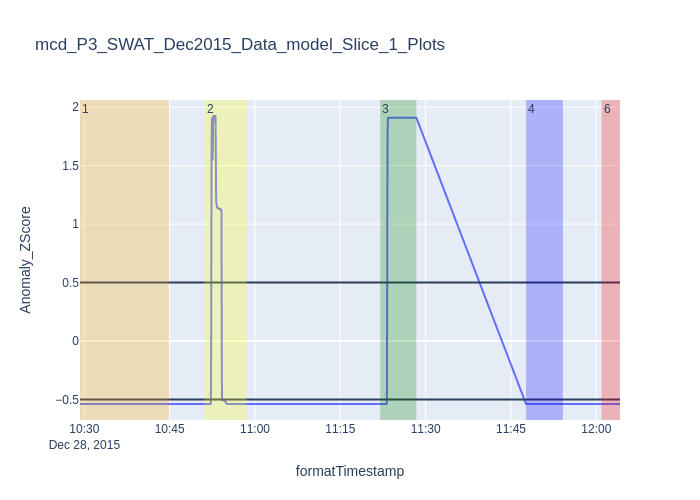
\includegraphics[width=0.46\linewidth]{images/PredictionPlots/mcd_P3_SWAT_Dec2015_Data_model_1_with_0.5.png}}%
            \hfill
        \subfloat[]{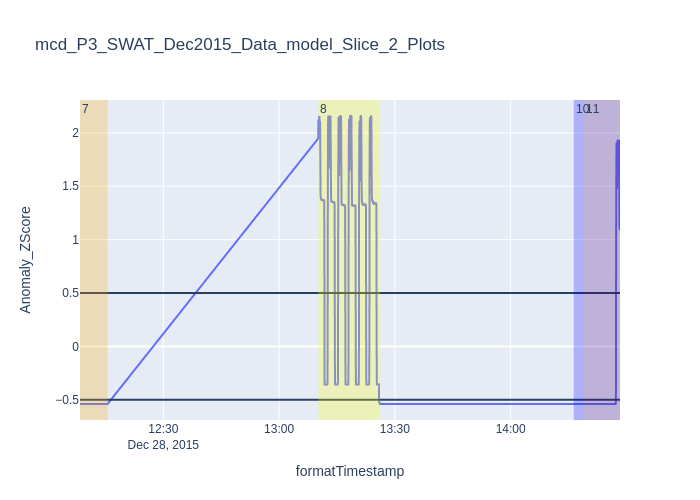
\includegraphics[width=0.48\linewidth]{images/PredictionPlots/mcd_P3_SWAT_Dec2015_Data_model_2_with_0.5.png}}
        
        \medskip
        \subfloat[]{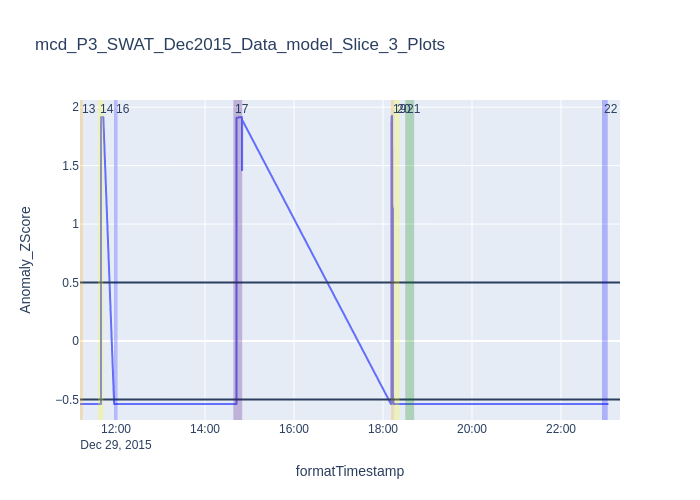
\includegraphics[width=0.48\linewidth]{images/PredictionPlots/mcd_P3_SWAT_Dec2015_Data_model_3_with_0.5.png}}%
            \hfill
        \subfloat[]{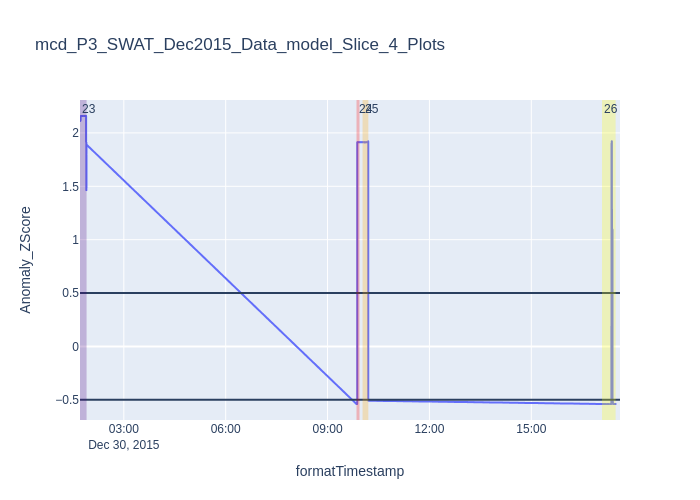
\includegraphics[width=0.48\linewidth]{images/PredictionPlots/mcd_P3_SWAT_Dec2015_Data_model_4_with_0.5.png}}
        
        \medskip
        \subfloat[]{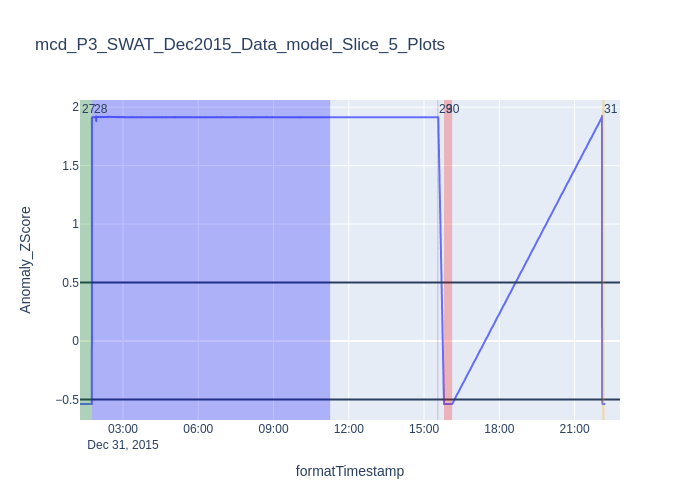
\includegraphics[width=0.48\linewidth]{images/PredictionPlots/mcd_P3_SWAT_Dec2015_Data_model_5_with_0.5.png}}%
            \hfill
        \subfloat[]{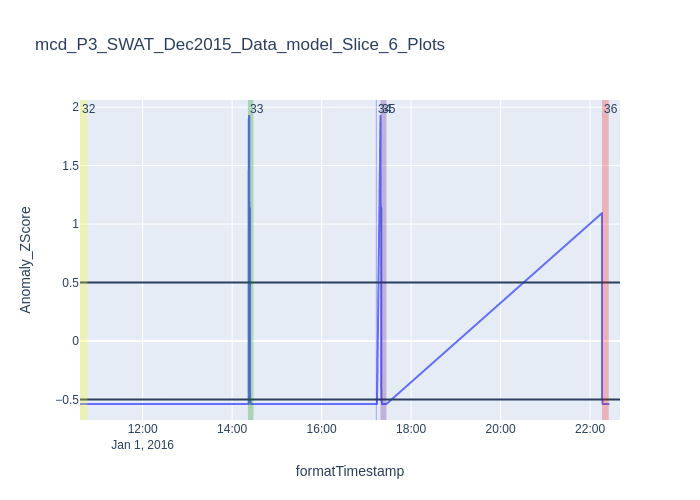
\includegraphics[width=0.48\linewidth]{images/PredictionPlots/mcd_P3_SWAT_Dec2015_Data_model_6_with_0.5.png}}
        
        \medskip
        \subfloat[]{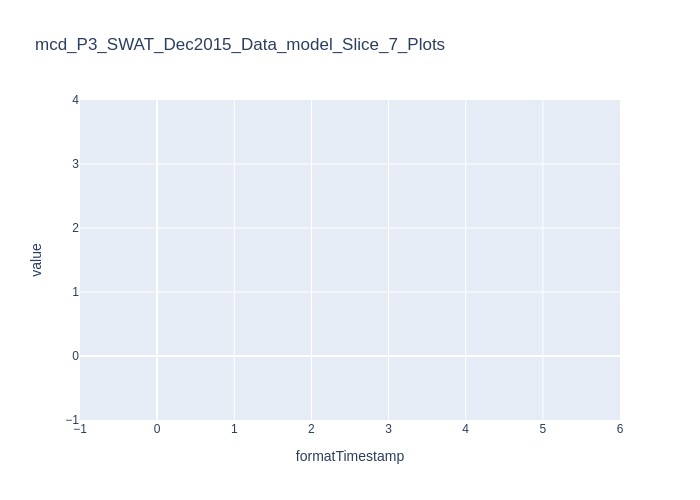
\includegraphics[width=0.48\linewidth]{images/PredictionPlots/mcd_P3_SWAT_Dec2015_Data_model_7_with_0.5.png}}%
            
        
        \caption{Minimum Covariance Determinant (MCD) Subsystem P3 model performance}
        \label{fig:MCDP3Plot}
    \end{figure}

    \begin{figure}[!ht]
    \subfloat[]{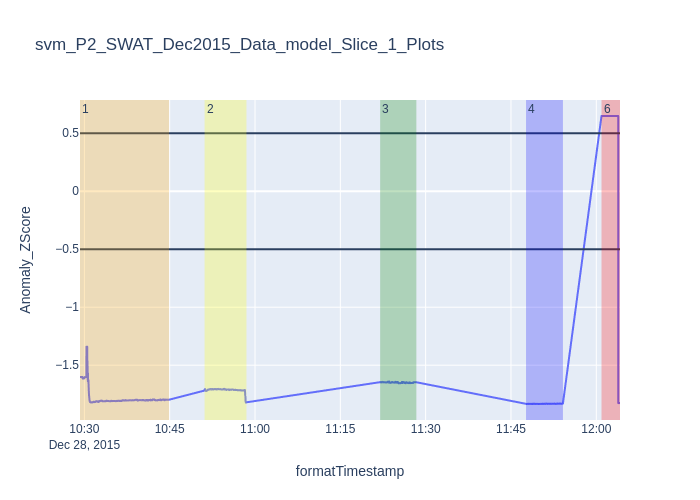
\includegraphics[width=0.46\linewidth]{images/PredictionPlots/svm_P2_SWAT_Dec2015_Data_model_1_with_0.5.png}}%
        \hfill
    \subfloat[]{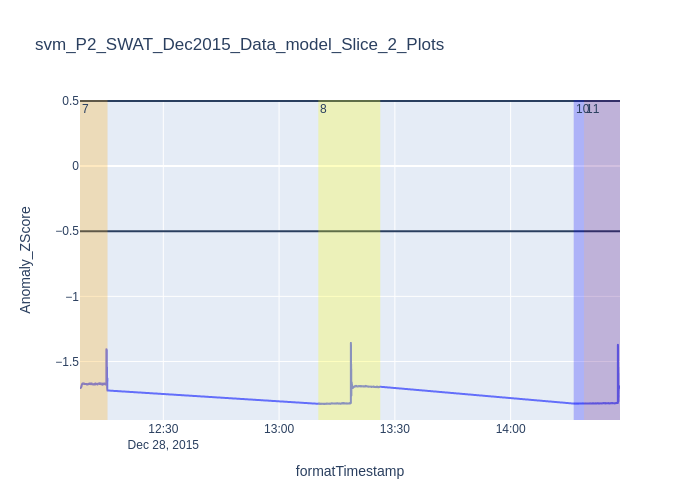
\includegraphics[width=0.48\linewidth]{images/PredictionPlots/svm_P2_SWAT_Dec2015_Data_model_2_with_0.5.png}}
    
    \medskip
    \subfloat[]{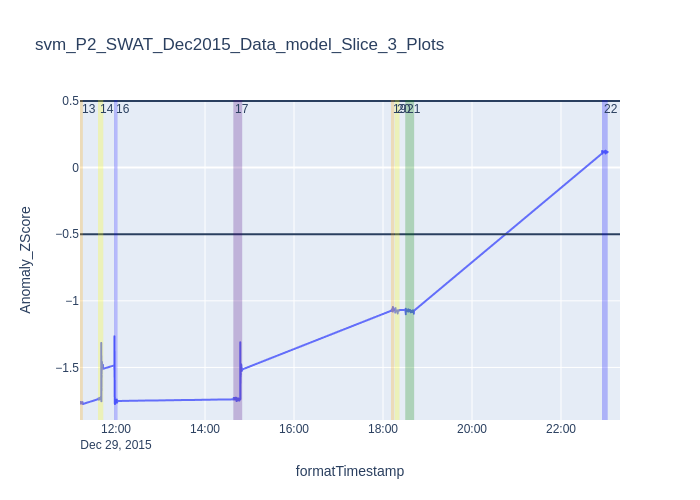
\includegraphics[width=0.48\linewidth]{images/PredictionPlots/svm_P2_SWAT_Dec2015_Data_model_3_with_0.5.png}}%
        \hfill
    \subfloat[]{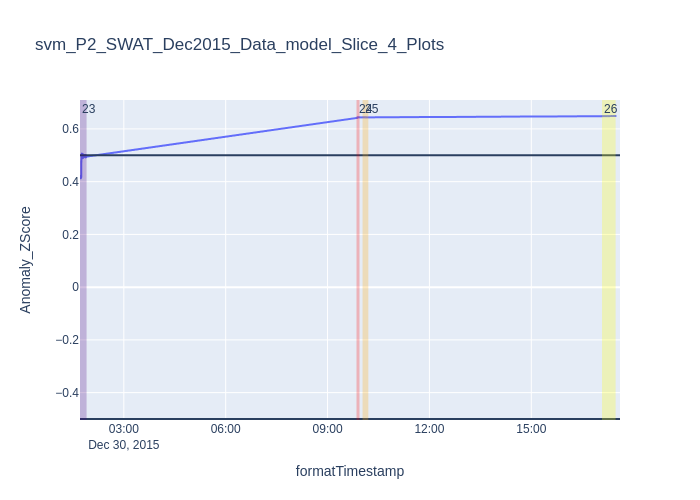
\includegraphics[width=0.48\linewidth]{images/PredictionPlots/svm_P2_SWAT_Dec2015_Data_model_4_with_0.5.png}}
    
    \medskip
    \subfloat[]{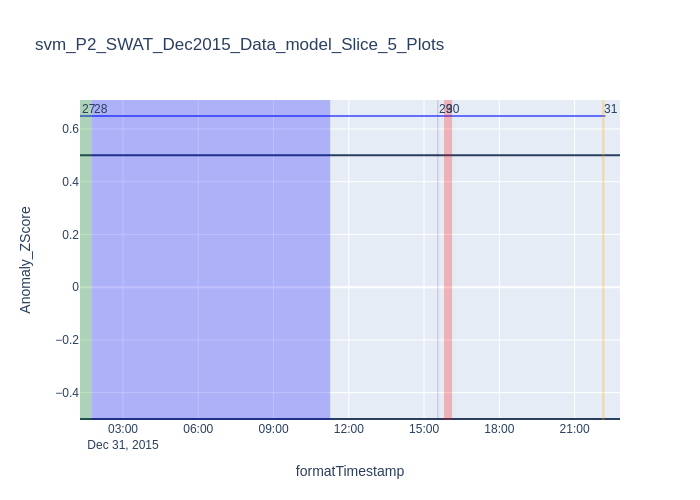
\includegraphics[width=0.48\linewidth]{images/PredictionPlots/svm_P2_SWAT_Dec2015_Data_model_5_with_0.5.png}}%
        \hfill
    \subfloat[]{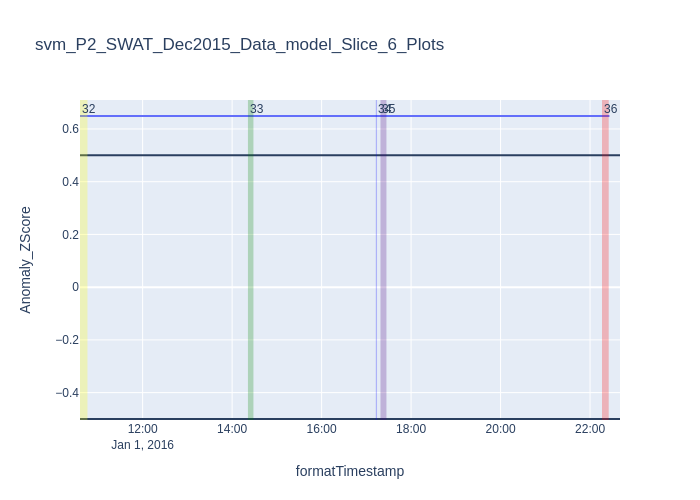
\includegraphics[width=0.48\linewidth]{images/PredictionPlots/svm_P2_SWAT_Dec2015_Data_model_6_with_0.5.png}}
    
    \medskip
    \subfloat[]{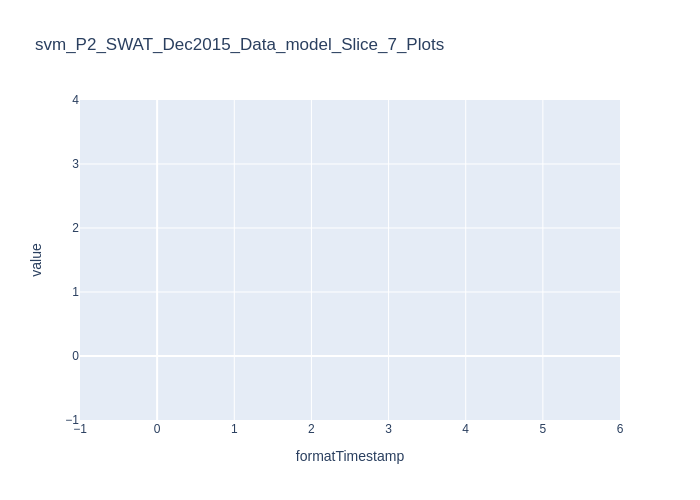
\includegraphics[width=0.48\linewidth]{images/PredictionPlots/svm_P2_SWAT_Dec2015_Data_model_7_with_0.5.png}}%
        
    
    \caption{SVM Subsystem P2 model performance}
    \label{fig:SVMP2Plot}
    \end{figure}

 \begin{figure}[!ht]
    \subfloat[]{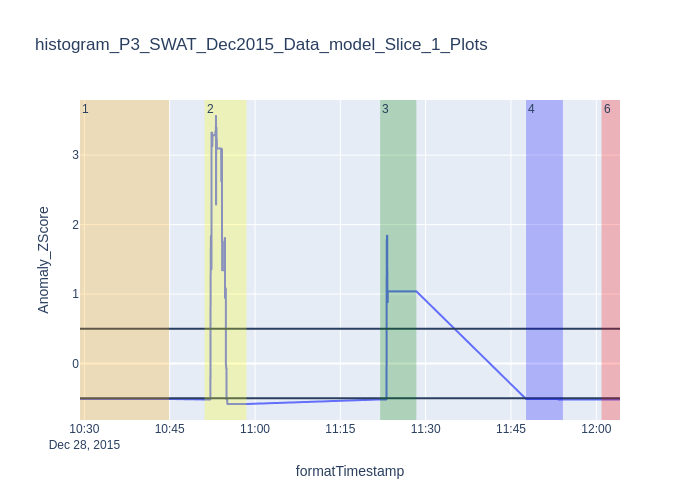
\includegraphics[width=0.46\linewidth]{images/PredictionPlots/histogram_P3_SWAT_Dec2015_Data_model_1_with_0.5.png}}%
        \hfill
    \subfloat[]{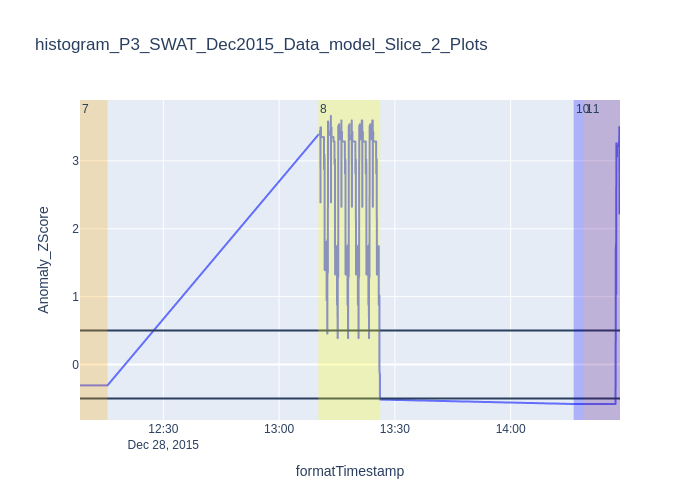
\includegraphics[width=0.48\linewidth]{images/PredictionPlots/histogram_P3_SWAT_Dec2015_Data_model_2_with_0.5.png}}
    
    \medskip
    \subfloat[]{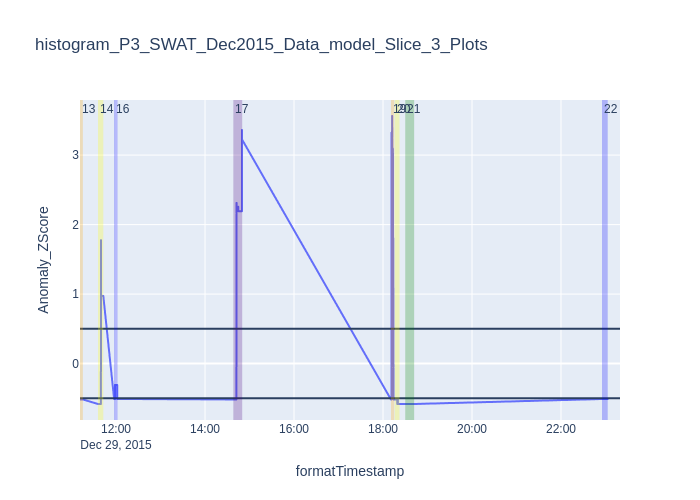
\includegraphics[width=0.48\linewidth]{images/PredictionPlots/histogram_P3_SWAT_Dec2015_Data_model_3_with_0.5.png}}%
        \hfill
    \subfloat[]{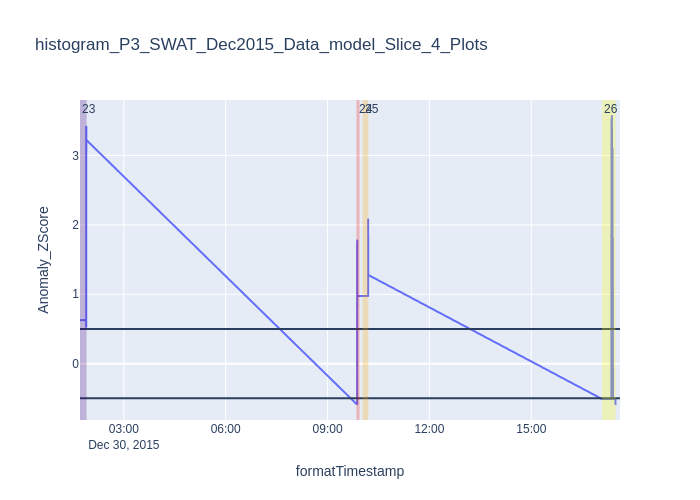
\includegraphics[width=0.48\linewidth]{images/PredictionPlots/histogram_P3_SWAT_Dec2015_Data_model_4_with_0.5.png}}
    
    \medskip
    \subfloat[]{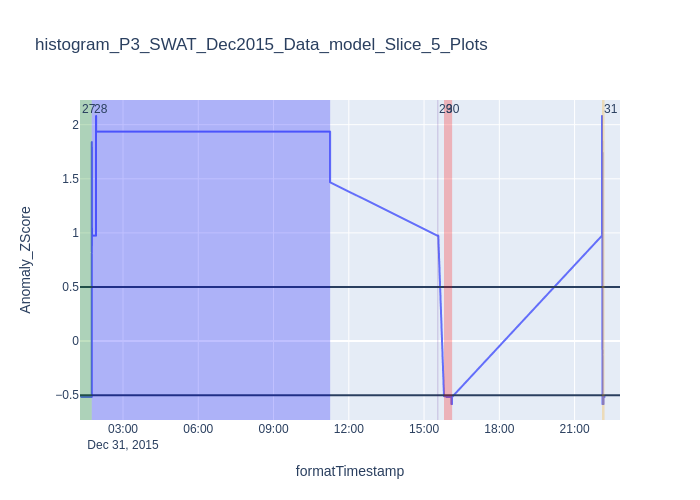
\includegraphics[width=0.48\linewidth]{images/PredictionPlots/histogram_P3_SWAT_Dec2015_Data_model_5_with_0.5.png}}%
        \hfill
    \subfloat[]{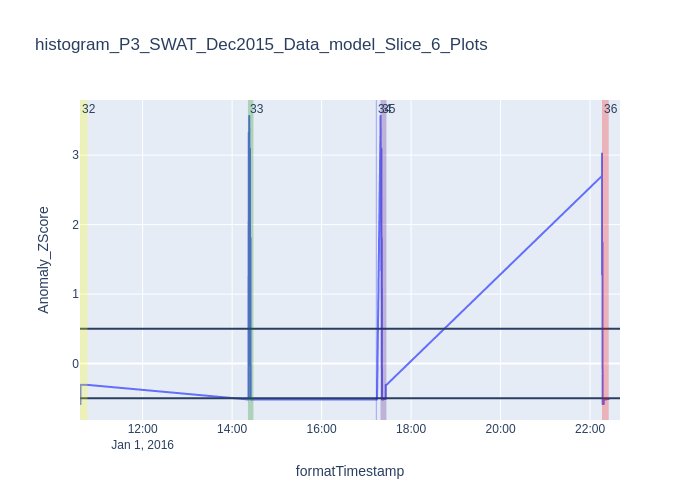
\includegraphics[width=0.48\linewidth]{images/PredictionPlots/histogram_P3_SWAT_Dec2015_Data_model_6_with_0.5.png}}
    
    \medskip
    \subfloat[]{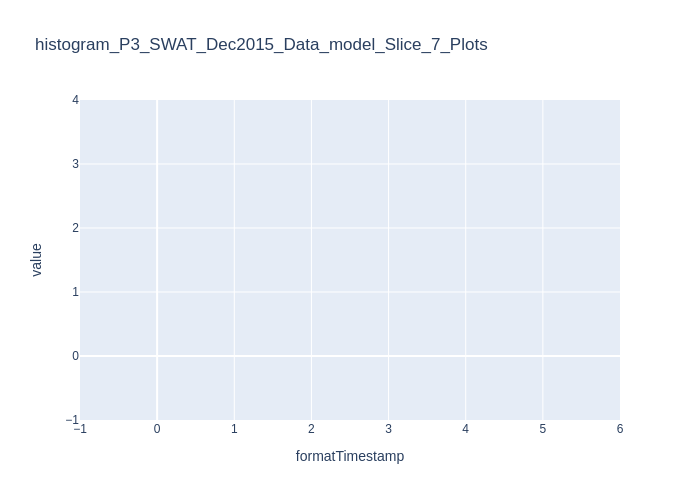
\includegraphics[width=0.48\linewidth]{images/PredictionPlots/histogram_P3_SWAT_Dec2015_Data_model_7_with_0.5.png}}%
        
    
    \caption{Histogram Subsystem P3 model performance}
    \label{fig:HistogramP3Plot}
    \end{figure}
 
 \begin{figure}[!ht]
    \subfloat[]{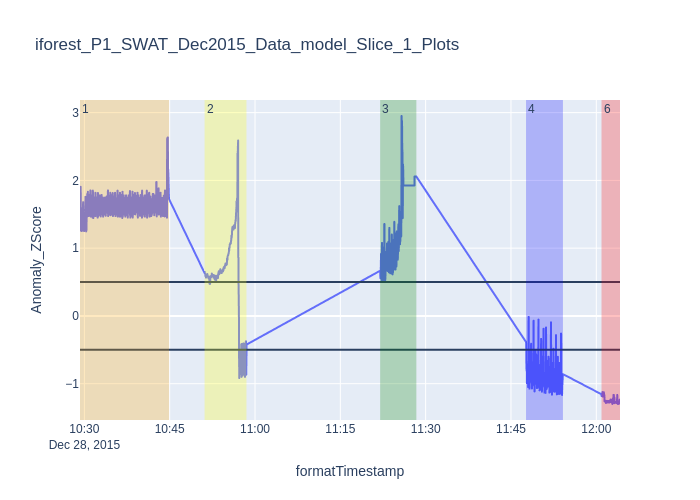
\includegraphics[width=0.46\linewidth]{images/PredictionPlots/iforest_P1_SWAT_Dec2015_Data_model_1_with_0.5.png}}%
        \hfill
    \subfloat[]{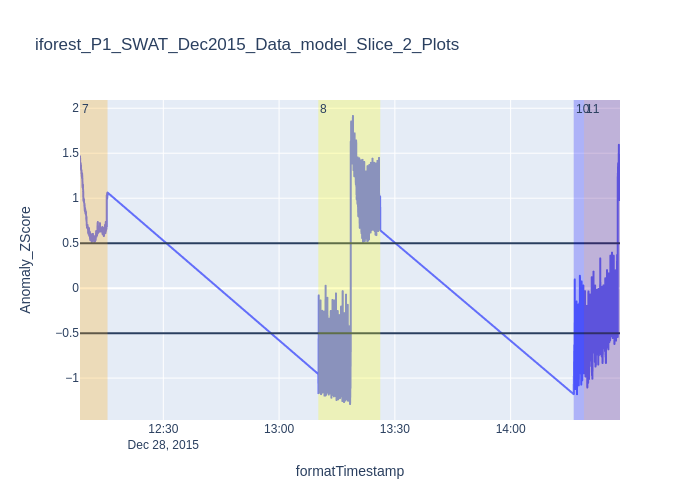
\includegraphics[width=0.48\linewidth]{images/PredictionPlots/iforest_P1_SWAT_Dec2015_Data_model_2_with_0.5.png}}
    
    \medskip
    \subfloat[]{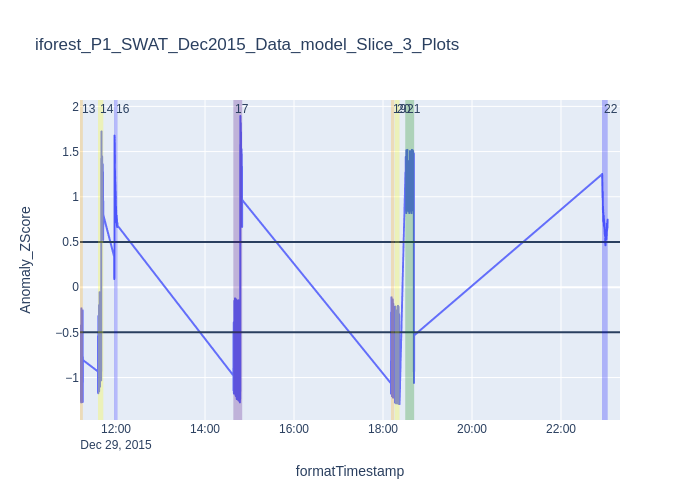
\includegraphics[width=0.48\linewidth]{images/PredictionPlots/iforest_P1_SWAT_Dec2015_Data_model_3_with_0.5.png}}%
        \hfill
    \subfloat[]{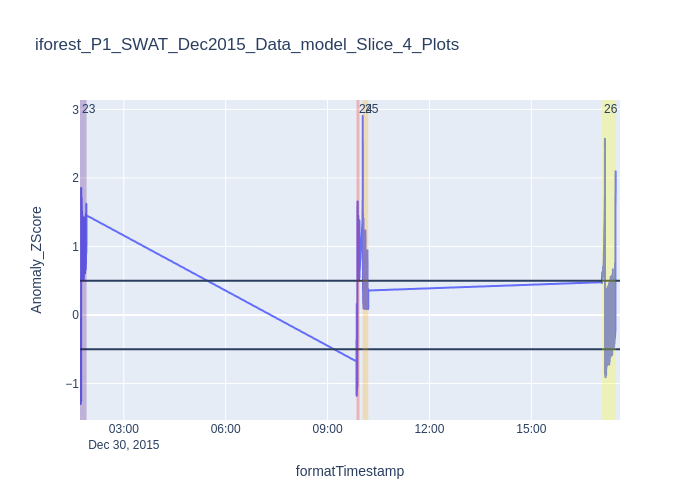
\includegraphics[width=0.48\linewidth]{images/PredictionPlots/iforest_P1_SWAT_Dec2015_Data_model_4_with_0.5.png}}
    
    \medskip
    \subfloat[]{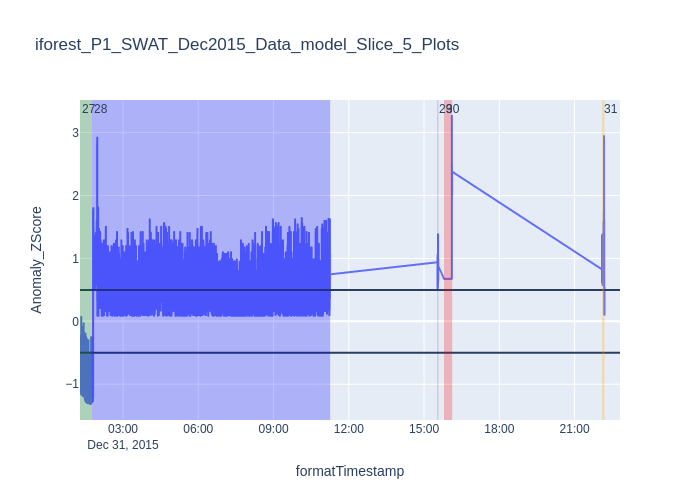
\includegraphics[width=0.48\linewidth]{images/PredictionPlots/iforest_P1_SWAT_Dec2015_Data_model_5_with_0.5.png}}%
        \hfill
    \subfloat[]{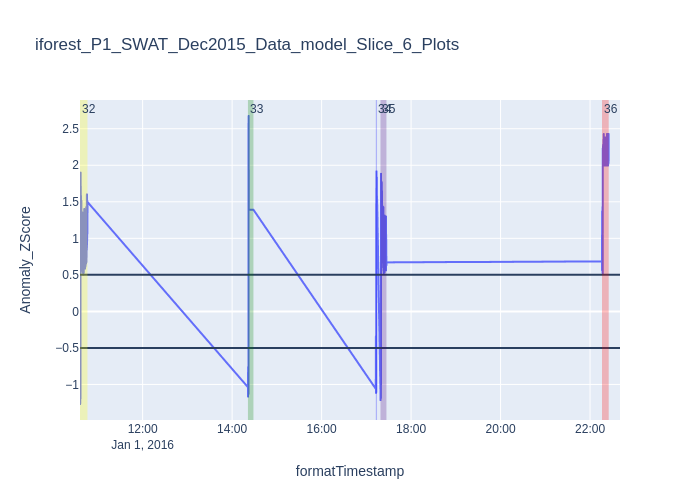
\includegraphics[width=0.48\linewidth]{images/PredictionPlots/iforest_P1_SWAT_Dec2015_Data_model_6_with_0.5.png}}
    
    \medskip
    \subfloat[]{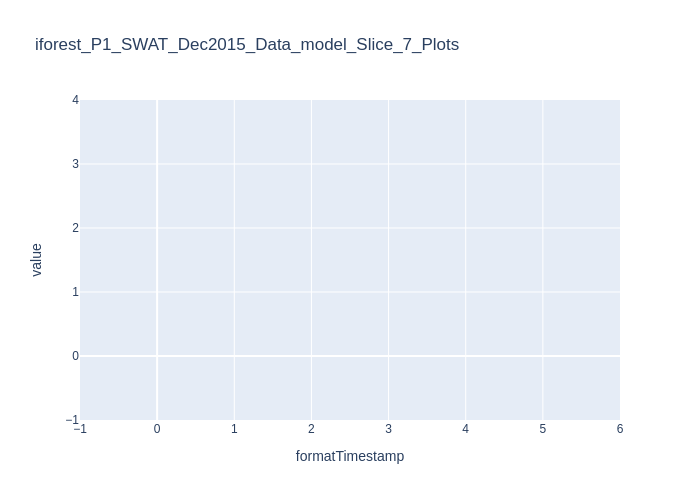
\includegraphics[width=0.48\linewidth]{images/PredictionPlots/iforest_P1_SWAT_Dec2015_Data_model_7_with_0.5.png}}%
        
    
    \caption{iforest Subsystem P1 model performance}
    \label{fig:iforestP1Plot}
    \end{figure}

    \begin{figure}[!ht]
        \caption{\textbf{Top 3 Performing Models by \% of Identified Attacks}}
        \label{fig:Top3ByIdentifiedAttacks}
            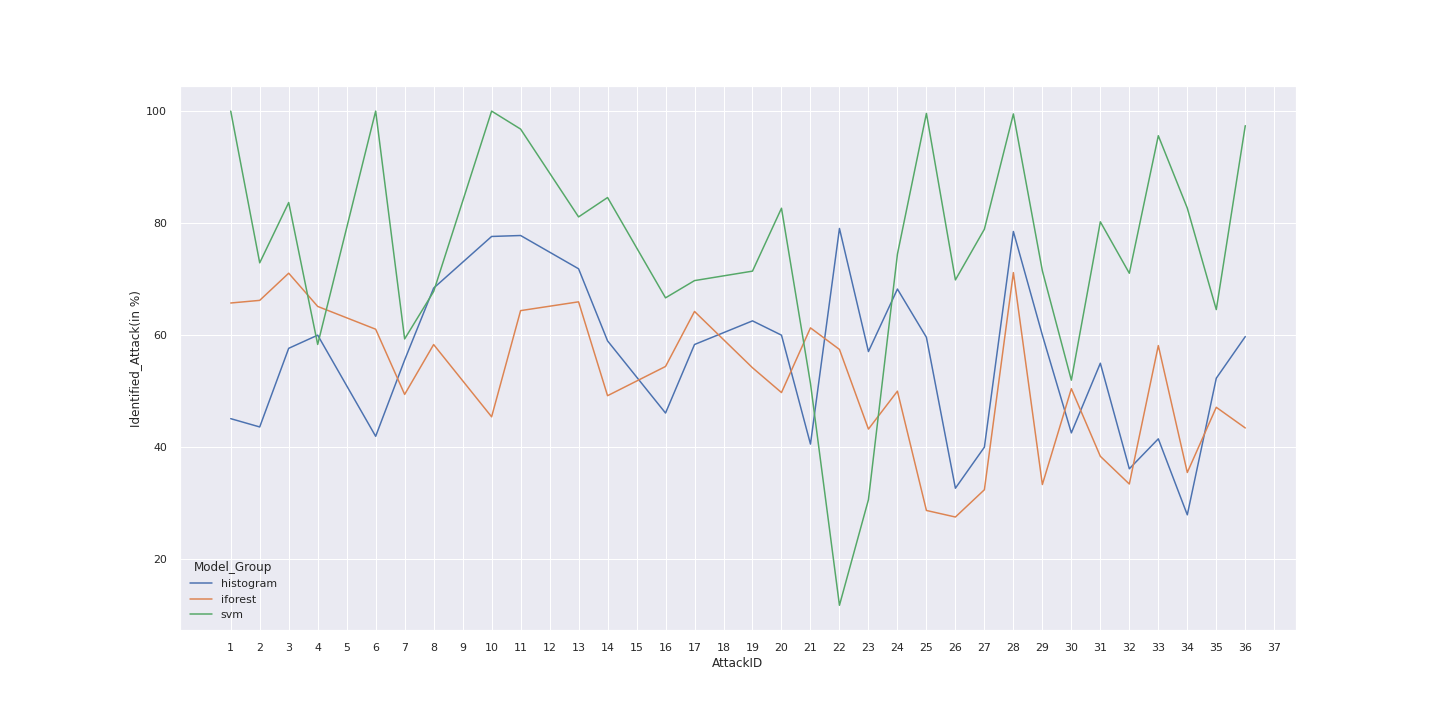
\includegraphics[width=1.0\textwidth]{images/ComparePlots/Top3ModelsByIdentifiedAttacks.png}
        \end{figure}

        \begin{figure}[h!]
        \caption{\textbf{Bottom 3 Performing Models by \% of Identified Attacks}}
        \label{fig:Bottom3ByIdentifiedAttacks}
            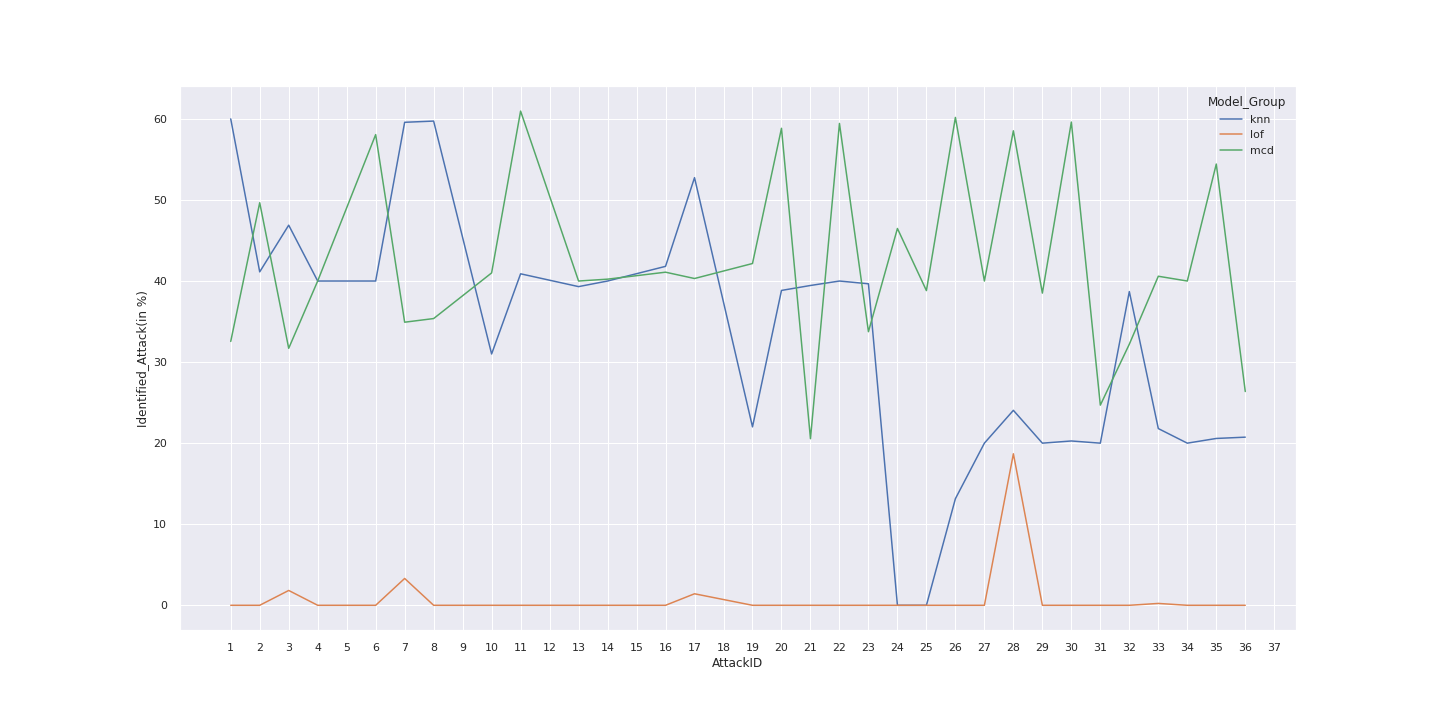
\includegraphics[width=1.0\textwidth]{images/ComparePlots/Bottom3ModelsByIdentifiedAttacks.png}
        \end{figure}


    \begin{figure}[!ht]
        \caption{\textbf{Top 3 Performing Models by Mean Of PropensityOfAttack (In Seconds)}}
        \label{fig:Top3ByPropensity}
            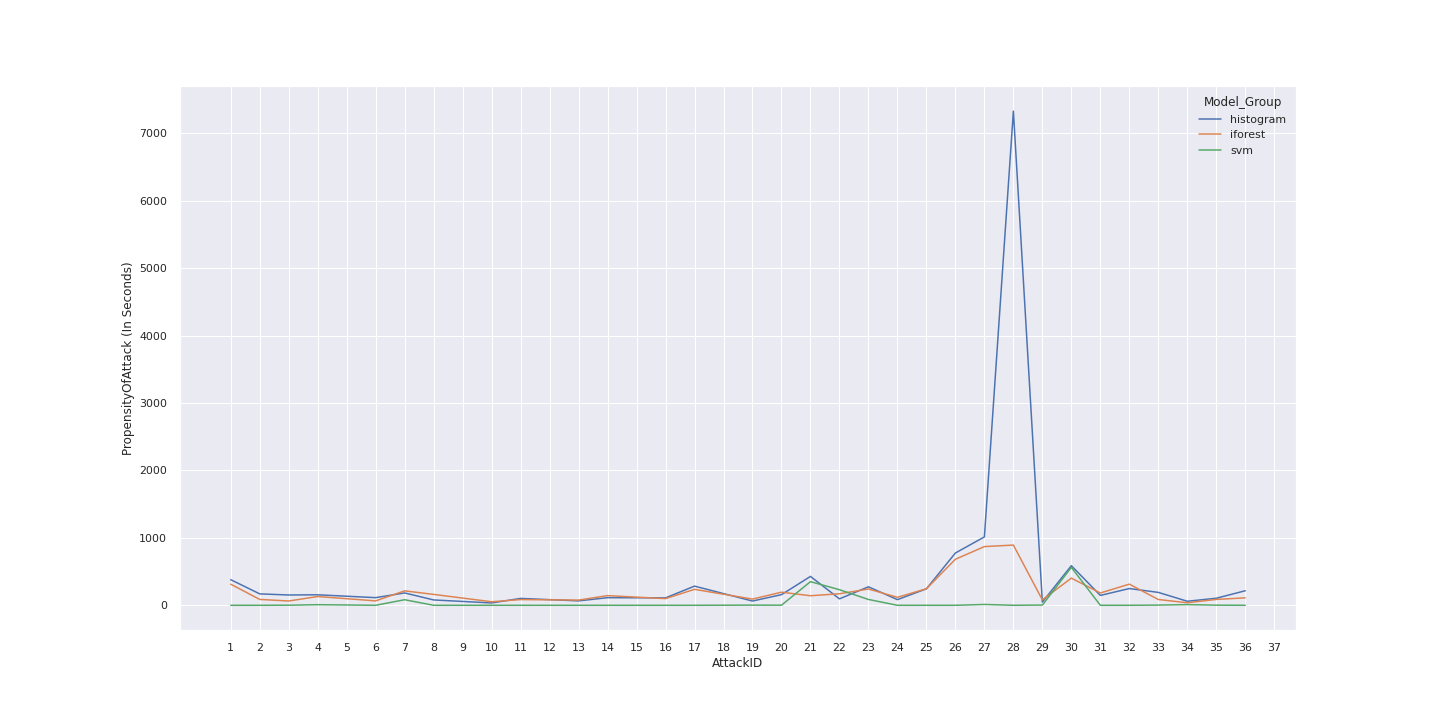
\includegraphics[width=1.0\textwidth]{images/ComparePlots/Top3ModelsByPropensity.png}
        \end{figure}

    \begin{figure}[!ht]
        \caption{\textbf{Bottom 3 Performing Models by Mean Of PropensityOfAttack (In Seconds)}}
        \label{fig:Bottom3ByPropensity}
            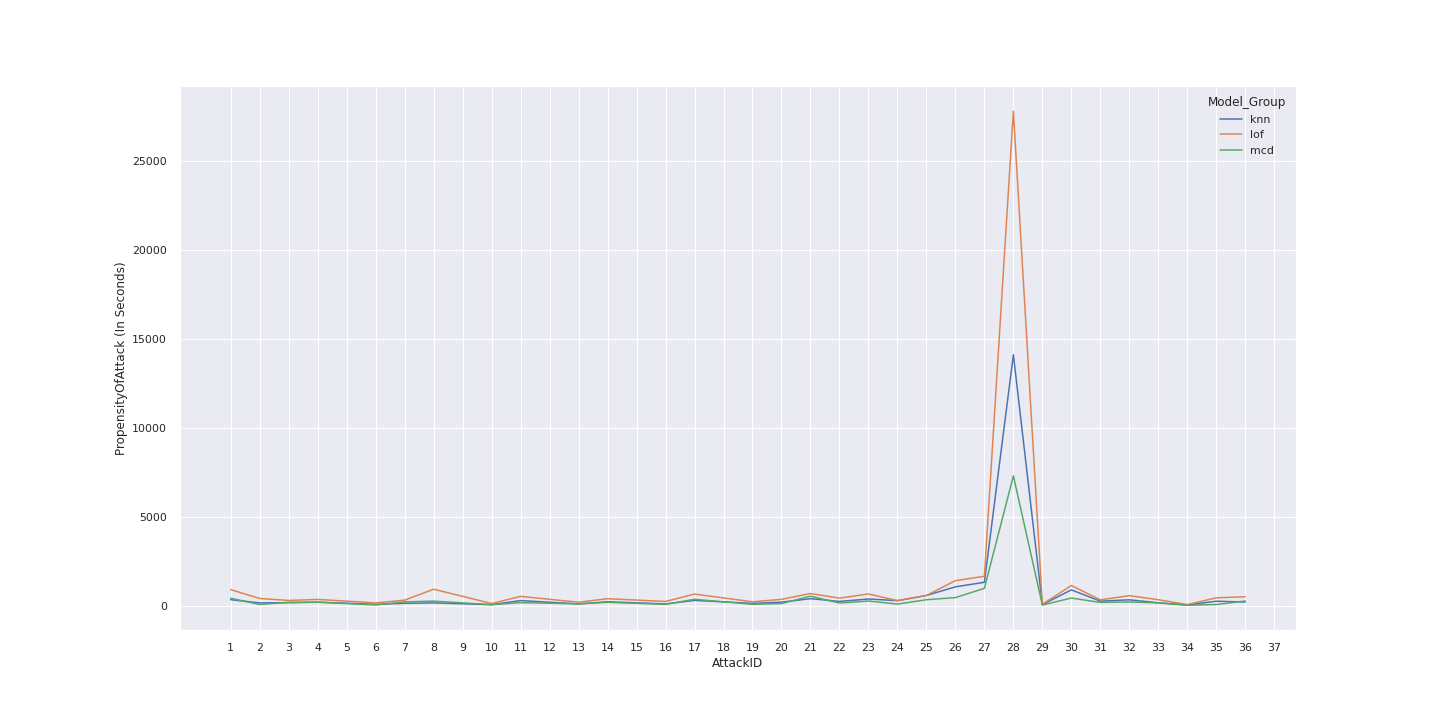
\includegraphics[width=1.0\textwidth]{images/ComparePlots/Bottom3ModelsByPropensity.png}
        \end{figure}
  
 \clearpage      
   
\subsection{Analysis on best performing ML algorithm and Models and Recommendations}
    \begin{enumerate}
        \item \textbf{Analysis on \% Of Identified Attacks}
        \begin{enumerate}
            
            \item We observed that OneSVM model has the best performance metrics (\textbf{\% of Identified Attacks: 90.62\%}). Please refer to Table  \ref{table:ModelGroupIdentifiedAttackPerformance}. Based on the underlying methodology of OneSVM, where it creates a non-linear decision boundary to separate two classes, It is not surprising that it consistently identifies the anomaly and performs the best. Please refer to Figure \ref{fig:SVMP2Plot}, where we have plotted OneSVM anomaly detection for the model trained on the sub-system P2. As well, OneSVM is able to identify the attack earliest as it has the lowest Propensity to identify the attacks. Please refer to Table \ref{table:ModelGroupPropensityPerformance}.
        
            \item We also plotted the Top 3 performing models by \% of Identified Attacks across all attacks (Table \ref{table:ModelGroupIdentifiedAttackPerformance} and Figure \ref{fig:Top3ByIdentifiedAttacks}: Attack 1 through Attack 41 - Between 28 December 2015 and 2nd-Jan-2016). We observe from the plot that OneSVM consistently identifies the attack better (higher) among all other models. Only for attacks 21 through 23 (between 29th December 2015 6.30 PM and 1.42 PM), OneSVM performance is worse than the  other models (Histogram, iForest, knn , and lof). This need to be looked at closely and analyzed further.
    
            \item Apart from OneSVM, the other two best-performing models are Histogram and iforest (Table \ref{table:ModelGroupIdentifiedAttackPerformance}). Histogram determines anomaly based on Count Statistics. The tail distribution of the Histogram is identified as Anomaly. Under Central Limit Theorem, for large Data Sizes, Histograms will converge to Gaussian distribution and the tail will be identified as an outlier. Hence, Histogram does a better job of identifying attacks. (\textbf{\% of Identified Attacks: 69.74\%})
    
            \item Apart from OneSVM and Histogram models (Table \ref{table:ModelGroupIdentifiedAttackPerformance}), the iforest  model detects anomalies in high dimensions by randomly selecting the value and then randomly selecting the split value between the maximum and minimum of the selected feature value. Anomalies will require a shorter path from the root. This is one of the best models for identifying Anomalies in high dimensions. In observed model performance, iforest does a good job of identifying Attacks (\textbf{\% of Identified Attacks: 63.91\%})
     
        \end{enumerate}

        \item \textbf{Analysis on individual models for \% Of Identified Attacks and Propensity (early detection)}
        \begin{enumerate}
            \item We also looked into the top three models' ability to identify the attacks and propensity of attacks (earliest to attacks) for a specific attack. We observe (Table \ref{table:ModelSingleAttackPerformanceIdentifiedAttackPercentage} and Table \ref{table:ModelSingleAttackPerformancePropensity}) that iforest (P1 Sub-system) and Histogram (P2 Sub-System)  identify 100\% of attacks within 0 Seconds (Propensity). This is quite impressive - given the robustness of models as we observe from Figure \ref{fig:HistogramP3Plot} and Figure \ref{fig:iforestP1Plot}. However,  across sub-systems and across all attacks, they do not have good performance metrics as we observe in Table \ref{table:ModelGroupIdentifiedAttackPerformance} , Table \ref{table:ModelGroupPropensityPerformance} ,and Figure \ref{fig:Top3ByIdentifiedAttacks}.

            \item Next, we looked into  the top three models' ability to identify the attacks and propensity of attacks (earliest to attacks) across all attacks for a specific sub-system model. We have a mixed-bag observation (Table \ref{table:ModelAcrossAttacksIdentifiedAttackPerformance} and Table \ref{table:ModelAcrossAttacksPropensity}). We expected OneSVM, Histogram, and SVM to perform better based on the performance metrics of Table \ref{table:ModelGroupIdentifiedAttackPerformance} and Table \ref{table:ModelGroupPropensityPerformance}. However, surprisingly MCD (P3 Sub-system) performed quite impressive for identified attacks (\textbf{\% of Identified Attacks: 99.27\% and Propensity : 0 Seconds}). We plotted Figure \ref{fig:MCDP3Plot} to observe its ability to identify the attacks. It appears that MCD (P3 Subsystems) features are densely located and hence its performance is stellar. We can state that if a particular dataset is densely clustered in high dimensions, Mahalanbosis distance will be quite effective in identifying dispersion and anomalies.  However,  across sub-systems and across all attacks, MCD does not have good performance metrics as we observe in Table \ref{table:ModelGroupIdentifiedAttackPerformance} ,and Figure \ref{fig:Bottom3ByIdentifiedAttacks}.
    
            \item We also plotted the Bottom 3 performing models by \% of Identified Attacks across all attacks (Table \ref{table:ModelGroupIdentifiedAttackPerformance} and Figure \ref{fig:Bottom3ByIdentifiedAttacks}: Attack 1 through Attack 41 - Between 28 December 2015 and 2nd-Jan-2016).All these models (KNN, MCD, and LOF) are inferior to OneSVM.  LOF (Local Outlier Factor) performs the worst as it has identified only 12\% (approx.) of attacks.LOF reflects a degree of an anomaly if an observation is different from the local density of neighbors obtained from the K-Nearest Neighbors. It appears that the data is quite sparsely distributed and hence LOF could not identify the attacks appropriately. 
    
            \item One of the worse performing models (Table \ref{table:ModelGroupIdentifiedAttackPerformance}), the Minimum Covariance Determinant (MCD) model detects anomalies in high dimensions by computing Mahalanbosis Distance(Based on underlying features). The broader the distribution of MCD, the probability of identifying anomalies are higher. In Our case, MCD does a bad job of identifying Attacks (\textbf{\% of Identified Attacks: 53.37\%})
     
        \end{enumerate}
        
        
        \item \textbf{Analysis on Propensity of Attacks (early detection)}
        \begin{enumerate}
            \item For Performance metrics in terms of Propensity of Attacks (earliest to identify), OneSVM performs the best (Please refer to Table \ref{table:ModelGroupPropensityPerformance} ) across all models. We expected it as OneSVM is quick to identify slight perturbations and detect anomalies. However, The minimum time to identify anomalies (Propensity) is \textbf{43 Seconds}, which is quite good. As we observe from (Figure \ref{fig:Top3ByPropensity}: the Top 3 performing Models by Means of Propensity (in Seconds) ), OneSVM propensity is close to zero seconds for all attacks but attacks 20 through 22 and attacks 29 through 31. We need to analyze it further.

            \item However, Performance metrics in terms of Propensity of Attacks (earliest to identify), Apart from OneSVM, other models (Please refer to table \ref{table:ModelGroupPropensityPerformance}) perform the worst (at least 5 times worse than the OneSVM Model). With these performance propensity metrics, apart from the OneSVM model, other models may not be acceptable for production-level anomaly detection systems. 
            
            \item As we Observe from Figure \ref{fig:Top3ByPropensity}- Top 3 Performing Models by Mean Of PropensityOfAttack (In Seconds), the iforest model is relatively better than the Histogram model. The iForest model performance degrades through attack 26 and attacks 29 - resulting in an overall bad propensity score \textbf{251.38 Seconds}.  However, for Attacks 24 through 29, Histogram performance degrades which needs to be analyzed further. It has impacted the mean of the Propensity score \textbf{451.88 Seconds}. 
    
            \item  As we Observe from Figure \ref{fig:Bottom3ByPropensity} - Bottom 3 Performing Models by Mean Of PropensityOfAttack (In Seconds), KNN, LOF, and MCD performances are quite bad. For Attacks 26 through 29, performance degrades need to be analyzed further. It has  impacted the mean of the Propensity score.
            
            \item  We observe (Table \ref{table:ModelGroupPropensityPerformance}, Figure \ref{fig:Top3ByPropensity}, and Figure \ref{fig:Bottom3ByPropensity}) that the best performance for Propensity (In Seconds) for identifying attacks is \textbf{OneSVM: 43 Seconds}. In production systems, we should be able to identify anomalies at the earliest (less than 10 seconds). The degradation of Propensity may be attributed to below :
            

            \begin{enumerate}
                \item We are assuming all records are real anomalies for a given attack. However, the impact of anomaly has latency and the actual impact will be further in time. It will require domain knowledge and thorough analysis. Hence, due to our expansionary assumptions, Propensity metrics degrade.
    
                \item As we observe from (Figure \ref{fig:Top3ByPropensity} and Figure \ref{fig:Bottom3ByPropensity} ), there are spikes in propensity across model groups - which need to be further analyzed.  and attacks 29 through 31. We need to analyze it further. This degradation has impacted the mean of the Propensity score (negatively)
     
            \end{enumerate}

            \item For all models and across sub-systems, we could not identify any attack data for Attack 37 through Attack 41 (2nd Jan 2016 between 11:17:02 and 13:13:02). We should have considered removing it from the analysis.
            
     
        \end{enumerate}
        
        
        \item \textbf{Anomaly detection is Inversely proportional to the threshold of Standard Deviation } Anomaly detection is sensitive to the threshold of standard deviation. Lower the standard deviation, we will be able to detect Anomalies higher (\% of Identified Attacks) and early (Propensity of Attacks (in Seconds)) As We Compare and contrast, Table \ref{table:ModelGroupIdentifiedAttackPerformance} \& Table \ref{table:ModelGroupPropensityPerformance} (for Standard deviation of 0.5) and Table \ref{table:ModelGroupIdentifiedAttackPerformanceFor1.0} \& Table \ref{table:ModelGroupPropensityPerformanceFor1.0} (for Standard deviation of 1.0), we observe that for Standard deviation 1, the detected Anomalies (\% of Identified Attacks) are lower and (Propensity of Attacks (in Seconds)) is higher for all models across subsystems. 

        \item \textbf{Recommendations :}
        \begin{enumerate}
            \item As mentioned in the assumption Section, the OneSVM model is quite compute/resource intensive and we could not train the model for Subsystems P\_3 through P\_6. 

            \item Based on our Analysis and the above Performance metrics tables (Table 1 and Table 2), we conclude that the Overall OneSVM model performed the best in terms of \% Of Identified Attacks (\textbf{90.62 \%}) and (Mean) Propensity of Attacks (\textbf{ 43.82 Seconds})

        
            \item Under this constraint and for Identifying \% Of Attacks and Propensity (early detection) of Attacks, we would like to recommend the OneSVM model for Anomaly detection.
    
            \item We are indifferent in recommending the Histogram or iForest model for Anomaly detection as they equally performed well.
    
            \item Based on empirical evidence (observed) during this experimentation, we are not recommending other models such as MCD, KNN , and LOF.
     
        \end{enumerate}
    \end{enumerate}

\subsection{Next Steps}
\begin{enumerate}
    \item Train the model across all remaining Sub-system models \ref{infraLimit} (Especially OneSVM) to ensure that OneSVM remains the preferred and recommended model
    \item Extend underlying models to other Systems such as WADI
    \item Pursue Other models other to achieve better performance such as (Prophet, XGBoost). We think that Time Series based model may be able to detect anomalies as it captures the correlation of the feature's distribution as a time series.
\end{enumerate}
% \end{enumerate}

\section{References:}
\begin{thebibliography}{9}
  \bibitem{one} \text{Temporal Execution Behavior for Host Anomaly Detection in Programmable Logic Controllers.} \href{https://ieeexplore.ieee.org/document/8832261}{https://ieeexplore.ieee.org/document/8832261}
  \bibitem{two} \text{A Dataset to Support Research in the Design of Secure Water Treatment Systems} \href{https://www.researchgate.net/publication/305809559}{https://www.researchgate.net/publication/305809559}
  
  \bibitem{three} \text{sklearn.neighbors.LocalOutlierFactor} \url{https://scikit-learn.org/stable/modules/generated/sklearn.neighbors.LocalOutlierFactor.html}
  
  \bibitem{four} \text{ADBench: Anomaly Detection Benchmark} \\ \url{https://www.andrew.cmu.edu/user/yuezhao2/papers/22-preprint-adbench.pdf}

  \bibitem{five} \text{Handbook of Anomaly Detection with Python Outlier Detection — (4) Isolated Forest} \\ \url{https://towardsdatascience.com/use-the-isolated-forest-with-pyod-3818eea68f08}

  \bibitem{six} \href{Minimum Covariance Determinant}
  \url{https://scikit-learn.org/stable/modules/covariance.html\#robust-covariance}

  \bibitem{seven} \text{Handbook of Anomaly Detection: With Python Outlier Detection — (6) OCSVM}
  \url{https://dataman-ai.medium.com/handbook-of-anomaly-detection-with-python-outlier-detection-6-ocsvm-f746dae9f450}

  \bibitem{eight} \text{Local Outlier Factor (LOF) — Algorithm for outlier identification} \url{https://towardsdatascience.com/local-outlier-factor-lof-algorithm-for-outlier-identification-8efb887d9843}

  \bibitem{nine} \text{Handbook of Anomaly Detection: with Python Outlier Detection — (2) HBOS} \url{https://medium.com/dataman-in-ai/anomaly-detection-with-histogram-based-outlier-detection-hbo-bc10ef52f23f}

  \bibitem{ten} \text{Handbook of Anomaly Detection: With Python Outlier Detection — (8) KNN} \url{https://medium.com/dataman-in-ai/anomaly-detection-with-pyod-b523fc47db9}

  \bibitem{eleven} \text{Anomaly Detection: — (11) Anomaly-Score} \url{https://scikit-learn.org/stable/modules/outlier_detection.html}

  \bibitem{twelve} \text{Novelty and Outlier Detection} \url{https://scikit-learn.org/stable/modules/outlier_detection.html}

  \bibitem{thirteen} \text{IsolationForest Example} \url{https://scikit-learn.org/stable/auto_examples/ensemble/plot_isolation_forest.html}

  \bibitem{fourteen} \text{Robust covariance estimation and Mahalanobis distances relevance} \url{https://scikit-learn.org/stable/auto_examples/covariance/plot_mahalanobis_distances.html#sphx-glr-auto-examples-covariance-plot-mahalanobis-distances-py}

  \bibitem{fifteen} \text{Covariance Estimation} \url{https://scikit-learn.org/stable/modules/covariance.html#robust-covariance}  

  \bibitem{sixteen} \text{Comparing anomaly detection algorithms for outlier detection on toy datasets}
  \url{https://scikit-learn.org/stable/auto_examples/miscellaneous/plot_anomaly_comparison.html}
  
\end{thebibliography}
\end{document}
